\documentclass[a4paperpaper,]{article}
\usepackage{lmodern}
\usepackage{svg}
\usepackage{amssymb,amsmath}
\usepackage{ifxetex,ifluatex}
\usepackage{fixltx2e} % provides \textsubscript
\ifnum 0\ifxetex 1\fi\ifluatex 1\fi=0 % if pdftex
  \usepackage[T1]{fontenc}
  \usepackage[utf8]{inputenc}
\else % if luatex or xelatex
  \ifxetex
    \usepackage{mathspec}
  \else
    \usepackage{fontspec}
  \fi
  \defaultfontfeatures{Ligatures=TeX,Scale=MatchLowercase}
\fi
% use upquote if available, for straight quotes in verbatim environments
\IfFileExists{upquote.sty}{\usepackage{upquote}}{}
% use microtype if available
\IfFileExists{microtype.sty}{%
\usepackage{microtype}
\UseMicrotypeSet[protrusion]{basicmath} % disable protrusion for tt fonts
}{}
\usepackage[a4paper,margin=2cm]{geometry}
\usepackage[unicode=true]{hyperref}
\hypersetup{
            pdftitle={Modeling Things},
            pdfborder={0 0 0},
            breaklinks=true}
\urlstyle{same}  % don't use monospace font for urls
\usepackage{natbib}
\bibliographystyle{plainnat}
\IfFileExists{parskip.sty}{%
\usepackage{parskip}
}{% else
\setlength{\parindent}{0pt}
\setlength{\parskip}{6pt plus 2pt minus 1pt}
}
\setcounter{secnumdepth}{5}


% set default figure placement to htbp
\makeatletter

\def\fps@figure{htbp}
\makeatother
\usepackage{graphicx}



\usepackage{amssymb} 
\usepackage{enumitem}
\usepackage{xcolor}
\usepackage{lipsum}
\usepackage{titlesec}

\providecommand{\tightlist}{%
  \setlength{\itemsep}{0pt}\setlength{\parskip}{0pt}}


\begin{document}


\title{Modeling Things}

\author{Neil D. Lawrence}

\date{2020-08-23}


\maketitle

\abstract{Machine learning solutions, in particular those based on deep
learning methods, form an underpinning of the current revolution in
``artificial intelligence'' that has dominated popular press headlines
and is having a significant influence on the wider tech agenda. In some
ways the these deep learning methods are radically new: they raise
questions about how we think of model regularization. Regularization
arises implicitly through the optimization. Yet in others they remain
rigidly traditional, and unsuited for an emerging world of unstructured,
streaming data. In this paper we relate these new methods to traditional
approaches and speculate on new directions that might take us beyond
modeling structured data.}

\newcommand{\tk}[1]{}
%\newcommand{\tk}[1]{\textbf{TK}: #1}
\newcommand{\Amatrix}{\mathbf{A}}
\newcommand{\KL}[2]{\text{KL}\left( #1\,\|\,#2 \right)}
\newcommand{\Kaast}{\kernelMatrix_{\mathbf{ \ast}\mathbf{ \ast}}}
\newcommand{\Kastu}{\kernelMatrix_{\mathbf{ \ast} \inducingVector}}
\newcommand{\Kff}{\kernelMatrix_{\mappingFunctionVector \mappingFunctionVector}}
\newcommand{\Kfu}{\kernelMatrix_{\mappingFunctionVector \inducingVector}}
\newcommand{\Kuast}{\kernelMatrix_{\inducingVector \bf\ast}}
\newcommand{\Kuf}{\kernelMatrix_{\inducingVector \mappingFunctionVector}}
\newcommand{\Kuu}{\kernelMatrix_{\inducingVector \inducingVector}}
\newcommand{\Kuui}{\Kuu^{-1}}
\newcommand{\Qaast}{\mathbf{Q}_{\bf \ast \ast}}
\newcommand{\Qastf}{\mathbf{Q}_{\ast \mappingFunction}}
\newcommand{\Qfast}{\mathbf{Q}_{\mappingFunctionVector \bf \ast}}
\newcommand{\Qff}{\mathbf{Q}_{\mappingFunctionVector \mappingFunctionVector}}
\newcommand{\aMatrix}{\mathbf{A}}
\newcommand{\aScalar}{a}
\newcommand{\aVector}{\mathbf{a}}
\newcommand{\acceleration}{a}
\newcommand{\bMatrix}{\mathbf{B}}
\newcommand{\bScalar}{b}
\newcommand{\bVector}{\mathbf{b}}
\newcommand{\basisFunc}{\phi}
\newcommand{\basisFuncVector}{\boldsymbol{ \basisFunc}}
\newcommand{\basisFunction}{\phi}
\newcommand{\basisLocation}{\mu}
\newcommand{\basisMatrix}{\boldsymbol{ \Phi}}
\newcommand{\basisScalar}{\basisFunction}
\newcommand{\basisVector}{\boldsymbol{ \basisFunction}}
\newcommand{\activationFunction}{\phi}
\newcommand{\activationMatrix}{\boldsymbol{ \Phi}}
\newcommand{\activationScalar}{\basisFunction}
\newcommand{\activationVector}{\boldsymbol{ \basisFunction}}
\newcommand{\bigO}{\mathcal{O}}
\newcommand{\binomProb}{\pi}
\newcommand{\cMatrix}{\mathbf{C}}
\newcommand{\cbasisMatrix}{\hat{\boldsymbol{ \Phi}}}
\newcommand{\cdataMatrix}{\hat{\dataMatrix}}
\newcommand{\cdataScalar}{\hat{\dataScalar}}
\newcommand{\cdataVector}{\hat{\dataVector}}
\newcommand{\centeredKernelMatrix}{\mathbf{ \MakeUppercase{\centeredKernelScalar}}}
\newcommand{\centeredKernelScalar}{b}
\newcommand{\centeredKernelVector}{\centeredKernelScalar}
\newcommand{\centeringMatrix}{\mathbf{H}}
\newcommand{\chiSquaredDist}[2]{\chi_{#1}^{2}\left(#2\right)}
\newcommand{\chiSquaredSamp}[1]{\chi_{#1}^{2}}
\newcommand{\conditionalCovariance}{\boldsymbol{ \Sigma}}
\newcommand{\coregionalizationMatrix}{\mathbf{B}}
\newcommand{\coregionalizationScalar}{b}
\newcommand{\coregionalizationVector}{\mathbf{ \coregionalizationScalar}}
\newcommand{\covDist}[2]{\text{cov}_{#2}\left(#1\right)}
\newcommand{\covSamp}[1]{\text{cov}\left(#1\right)}
\newcommand{\covarianceScalar}{c}
\newcommand{\covarianceVector}{\mathbf{ \covarianceScalar}}
\newcommand{\covarianceMatrix}{\mathbf{C}}
\newcommand{\covarianceMatrixTwo}{\boldsymbol{ \Sigma}}
\newcommand{\croupierScalar}{s}
\newcommand{\croupierVector}{\mathbf{ \croupierScalar}}
\newcommand{\croupierMatrix}{\mathbf{ \MakeUppercase{\croupierScalar}}}
\newcommand{\dataDim}{p}
\newcommand{\dataIndex}{i}
\newcommand{\dataIndexTwo}{j}
\newcommand{\dataMatrix}{\mathbf{Y}}
\newcommand{\dataScalar}{y}
\newcommand{\dataSet}{\mathcal{D}}
\newcommand{\dataStd}{\sigma}
\newcommand{\dataVector}{\mathbf{ \dataScalar}}
\newcommand{\decayRate}{d}
\newcommand{\degreeMatrix}{\mathbf{ \MakeUppercase{\degreeScalar}}}
\newcommand{\degreeScalar}{d}
\newcommand{\degreeVector}{\mathbf{ \degreeScalar}}
% Already defined by latex
%\newcommand{\det}[1]{\left|#1\right|}
\newcommand{\diag}[1]{\text{diag}\left(#1\right)}
\newcommand{\diagonalMatrix}{\mathbf{D}}
\newcommand{\diff}[2]{\frac{\text{d}#1}{\text{d}#2}}
\newcommand{\diffTwo}[2]{\frac{\text{d}^2#1}{\text{d}#2^2}}
\newcommand{\displacement}{x}
\newcommand{\displacementVector}{\textbf{\displacement}}
\newcommand{\distanceMatrix}{\mathbf{ \MakeUppercase{\distanceScalar}}}
\newcommand{\distanceScalar}{d}
\newcommand{\distanceVector}{\mathbf{ \distanceScalar}}
\newcommand{\eigenvaltwo}{\ell}
\newcommand{\eigenvaltwoMatrix}{\mathbf{L}}
\newcommand{\eigenvaltwoVector}{\mathbf{l}}
\newcommand{\eigenvalue}{\lambda}
\newcommand{\eigenvalueMatrix}{\boldsymbol{ \Lambda}}
\newcommand{\eigenvalueVector}{\boldsymbol{ \lambda}}
\newcommand{\eigenvector}{\mathbf{ \eigenvectorScalar}}
\newcommand{\eigenvectorMatrix}{\mathbf{U}}
\newcommand{\eigenvectorScalar}{u}
\newcommand{\eigenvectwo}{\mathbf{v}}
\newcommand{\eigenvectwoMatrix}{\mathbf{V}}
\newcommand{\eigenvectwoScalar}{v}
\newcommand{\entropy}[1]{\mathcal{H}\left(#1\right)}
\newcommand{\errorFunction}{E}
\newcommand{\expDist}[2]{\left<#1\right>_{#2}}
\newcommand{\expSamp}[1]{\left<#1\right>}
\newcommand{\expectation}[1]{\left\langle #1 \right\rangle }
\newcommand{\expectationDist}[2]{\left\langle #1 \right\rangle _{#2}}
\newcommand{\expectedDistanceMatrix}{\mathcal{D}}
\newcommand{\eye}{\mathbf{I}}
\newcommand{\fantasyDim}{r}
\newcommand{\fantasyMatrix}{\mathbf{ \MakeUppercase{\fantasyScalar}}}
\newcommand{\fantasyScalar}{z}
\newcommand{\fantasyVector}{\mathbf{ \fantasyScalar}}
\newcommand{\featureStd}{\varsigma}
\newcommand{\gammaCdf}[3]{\mathcal{GAMMA CDF}\left(#1|#2,#3\right)}
\newcommand{\gammaDist}[3]{\mathcal{G}\left(#1|#2,#3\right)}
\newcommand{\gammaSamp}[2]{\mathcal{G}\left(#1,#2\right)}
\newcommand{\gaussianDist}[3]{\mathcal{N}\left(#1|#2,#3\right)}
\newcommand{\gaussianSamp}[2]{\mathcal{N}\left(#1,#2\right)}
\newcommand{\given}{|}
\newcommand{\half}{\frac{1}{2}}
\newcommand{\heaviside}{H}
\newcommand{\hiddenMatrix}{\mathbf{ \MakeUppercase{\hiddenScalar}}}
\newcommand{\hiddenScalar}{h}
\newcommand{\hiddenVector}{\mathbf{ \hiddenScalar}}
\newcommand{\identityMatrix}{\eye}
\newcommand{\inducingInputScalar}{z}
\newcommand{\inducingInputVector}{\mathbf{ \inducingInputScalar}}
\newcommand{\inducingInputMatrix}{\mathbf{Z}}
\newcommand{\inducingScalar}{u}
\newcommand{\inducingVector}{\mathbf{ \inducingScalar}}
\newcommand{\inducingMatrix}{\mathbf{U}}
\newcommand{\inlineDiff}[2]{\text{d}#1/\text{d}#2}
\newcommand{\inputDim}{q}
\newcommand{\inputMatrix}{\mathbf{X}}
\newcommand{\inputScalar}{x}
\newcommand{\inputSpace}{\mathcal{X}}
\newcommand{\inputVals}{\inputVector}
\newcommand{\inputVector}{\mathbf{ \inputScalar}}
\newcommand{\iterNum}{k}
\newcommand{\kernel}{\kernelScalar}
\newcommand{\kernelMatrix}{\mathbf{K}}
\newcommand{\kernelScalar}{k}
\newcommand{\kernelVector}{\mathbf{ \kernelScalar}}
\newcommand{\kff}{\kernelScalar_{\mappingFunction \mappingFunction}}
\newcommand{\kfu}{\kernelVector_{\mappingFunction \inducingScalar}}
\newcommand{\kuf}{\kernelVector_{\inducingScalar \mappingFunction}}
\newcommand{\kuu}{\kernelVector_{\inducingScalar \inducingScalar}}
\newcommand{\lagrangeMultiplier}{\lambda}
\newcommand{\lagrangeMultiplierMatrix}{\boldsymbol{ \Lambda}}
\newcommand{\lagrangian}{L}
\newcommand{\laplacianFactor}{\mathbf{ \MakeUppercase{\laplacianFactorScalar}}}
\newcommand{\laplacianFactorScalar}{m}
\newcommand{\laplacianFactorVector}{\mathbf{ \laplacianFactorScalar}}
\newcommand{\laplacianMatrix}{\mathbf{L}}
\newcommand{\laplacianScalar}{\ell}
\newcommand{\laplacianVector}{\mathbf{ \ell}}
\newcommand{\latentDim}{q}
\newcommand{\latentDistanceMatrix}{\boldsymbol{ \Delta}}
\newcommand{\latentDistanceScalar}{\delta}
\newcommand{\latentDistanceVector}{\boldsymbol{ \delta}}
\newcommand{\latentForce}{f}
\newcommand{\latentFunction}{u}
\newcommand{\latentFunctionVector}{\mathbf{ \latentFunction}}
\newcommand{\latentFunctionMatrix}{\mathbf{ \MakeUppercase{\latentFunction}}}
\newcommand{\latentIndex}{j}
\newcommand{\latentScalar}{z}
\newcommand{\latentVector}{\mathbf{ \latentScalar}}
\newcommand{\latentMatrix}{\mathbf{Z}}
\newcommand{\learnRate}{\eta}
\newcommand{\lengthScale}{\ell}
\newcommand{\rbfWidth}{\ell}
\newcommand{\likelihoodBound}{\mathcal{L}}
\newcommand{\likelihoodFunction}{L}
\newcommand{\locationScalar}{\mu}
\newcommand{\locationVector}{\boldsymbol{ \locationScalar}}
\newcommand{\locationMatrix}{\mathbf{M}}
\newcommand{\variance}[1]{\text{var}\left( #1 \right)}
\newcommand{\mappingFunction}{f}
\newcommand{\mappingFunctionMatrix}{\mathbf{F}}
\newcommand{\mappingFunctionTwo}{g}
\newcommand{\mappingFunctionTwoMatrix}{\mathbf{G}}
\newcommand{\mappingFunctionTwoVector}{\mathbf{ \mappingFunctionTwo}}
\newcommand{\mappingFunctionVector}{\mathbf{ \mappingFunction}}
\newcommand{\scaleScalar}{s}
\newcommand{\mappingScalar}{w}
\newcommand{\mappingVector}{\mathbf{ \mappingScalar}}
\newcommand{\mappingMatrix}{\mathbf{W}}
\newcommand{\mappingScalarTwo}{v}
\newcommand{\mappingVectorTwo}{\mathbf{ \mappingScalarTwo}}
\newcommand{\mappingMatrixTwo}{\mathbf{V}}
\newcommand{\maxIters}{K}
\newcommand{\meanMatrix}{\mathbf{M}}
\newcommand{\meanScalar}{\mu}
\newcommand{\meanTwoMatrix}{\mathbf{M}}
\newcommand{\meanTwoScalar}{m}
\newcommand{\meanTwoVector}{\mathbf{ \meanTwoScalar}}
\newcommand{\meanVector}{\boldsymbol{ \meanScalar}}
\newcommand{\mrnaConcentration}{m}
\newcommand{\naturalFrequency}{\omega}
\newcommand{\neighborhood}[1]{\mathcal{N}\left( #1 \right)}
\newcommand{\neilurl}{http://inverseprobability.com/}
\newcommand{\noiseMatrix}{\boldsymbol{ E}}
\newcommand{\noiseScalar}{\epsilon}
\newcommand{\noiseVector}{\boldsymbol{ \epsilon}}
\newcommand{\norm}[1]{\left\Vert #1 \right\Vert}
\newcommand{\normalizedLaplacianMatrix}{\hat{\mathbf{L}}}
\newcommand{\normalizedLaplacianScalar}{\hat{\ell}}
\newcommand{\normalizedLaplacianVector}{\hat{\mathbf{ \ell}}}
\newcommand{\numActive}{m}
\newcommand{\numBasisFunc}{m}
\newcommand{\numComponents}{m}
\newcommand{\numComps}{K}
\newcommand{\numData}{n}
\newcommand{\numFeatures}{K}
\newcommand{\numHidden}{h}
\newcommand{\numInducing}{m}
\newcommand{\numLayers}{\ell}
\newcommand{\numNeighbors}{K}
\newcommand{\numSequences}{s}
\newcommand{\numSuccess}{s}
\newcommand{\numTasks}{m}
\newcommand{\numTime}{T}
\newcommand{\numTrials}{S}
\newcommand{\outputIndex}{j}
\newcommand{\paramVector}{\boldsymbol{ \theta}}
\newcommand{\parameterMatrix}{\boldsymbol{ \Theta}}
\newcommand{\parameterScalar}{\theta}
\newcommand{\parameterVector}{\boldsymbol{ \parameterScalar}}
\newcommand{\partDiff}[2]{\frac{\partial#1}{\partial#2}}
\newcommand{\precisionScalar}{j}
\newcommand{\precisionVector}{\mathbf{ \precisionScalar}}
\newcommand{\precisionMatrix}{\mathbf{J}}
\newcommand{\pseudotargetScalar}{\widetilde{y}}
\newcommand{\pseudotargetVector}{\mathbf{ \pseudotargetScalar}}
\newcommand{\pseudotargetMatrix}{\mathbf{ \widetilde{Y}}}
\newcommand{\rank}[1]{\text{rank}\left(#1\right)}
\newcommand{\rayleighDist}[2]{\mathcal{R}\left(#1|#2\right)}
\newcommand{\rayleighSamp}[1]{\mathcal{R}\left(#1\right)}
\newcommand{\responsibility}{r}
\newcommand{\rotationScalar}{r}
\newcommand{\rotationVector}{\mathbf{ \rotationScalar}}
\newcommand{\rotationMatrix}{\mathbf{R}}
\newcommand{\sampleCovScalar}{s}
\newcommand{\sampleCovVector}{\mathbf{ \sampleCovScalar}}
\newcommand{\sampleCovMatrix}{\mathbf{s}}
\newcommand{\scalarProduct}[2]{\left\langle{#1},{#2}\right\rangle}
\newcommand{\sign}[1]{\text{sign}\left(#1\right)}
\newcommand{\sigmoid}[1]{\sigma\left(#1\right)}
\newcommand{\singularvalue}{\ell}
\newcommand{\singularvalueMatrix}{\mathbf{L}}
\newcommand{\singularvalueVector}{\mathbf{l}}
\newcommand{\sorth}{\mathbf{u}}
\newcommand{\spar}{\lambda}
\newcommand{\trace}[1]{\text{tr}\left(#1\right)}
\newcommand{\BasalRate}{B}
\newcommand{\DampingCoefficient}{C}
\newcommand{\DecayRate}{D}
\newcommand{\Displacement}{X}
\newcommand{\LatentForce}{F}
\newcommand{\Mass}{M}
\newcommand{\Sensitivity}{S}
\newcommand{\basalRate}{b}
\newcommand{\dampingCoefficient}{c}
\newcommand{\mass}{m}
\newcommand{\sensitivity}{s}
\newcommand{\springScalar}{\kappa}
\newcommand{\springVector}{\boldsymbol{ \kappa}}
\newcommand{\springMatrix}{\boldsymbol{ \mathcal{K}}}
\newcommand{\tfConcentration}{p}
\newcommand{\tfDecayRate}{\delta}
\newcommand{\tfMrnaConcentration}{f}
\newcommand{\tfVector}{\mathbf{ \tfConcentration}}
\newcommand{\velocity}{v}
\newcommand{\sufficientStatsScalar}{g}
\newcommand{\sufficientStatsVector}{\mathbf{ \sufficientStatsScalar}}
\newcommand{\sufficientStatsMatrix}{\mathbf{G}}
\newcommand{\switchScalar}{s}
\newcommand{\switchVector}{\mathbf{ \switchScalar}}
\newcommand{\switchMatrix}{\mathbf{S}}
\newcommand{\tr}[1]{\text{tr}\left(#1\right)}
\newcommand{\loneNorm}[1]{\left\Vert #1 \right\Vert_1}
\newcommand{\ltwoNorm}[1]{\left\Vert #1 \right\Vert_2}
\newcommand{\onenorm}[1]{\left\vert#1\right\vert_1}
\newcommand{\twonorm}[1]{\left\Vert #1 \right\Vert}
\newcommand{\vScalar}{v}
\newcommand{\vVector}{\mathbf{v}}
\newcommand{\vMatrix}{\mathbf{V}}
\newcommand{\varianceDist}[2]{\text{var}_{#2}\left( #1 \right)}
% Already defined by latex
%\newcommand{\vec}{#1:}
\newcommand{\vecb}[1]{\left(#1\right):}
\newcommand{\weightScalar}{w}
\newcommand{\weightVector}{\mathbf{ \weightScalar}}
\newcommand{\weightMatrix}{\mathbf{W}}
\newcommand{\weightedAdjacencyMatrix}{\mathbf{A}}
\newcommand{\weightedAdjacencyScalar}{a}
\newcommand{\weightedAdjacencyVector}{\mathbf{ \weightedAdjacencyScalar}}
\newcommand{\onesVector}{\mathbf{1}}
\newcommand{\zerosVector}{\mathbf{0}}


%%%%%%%%%% Start Body %%%%%%%%%%

\definecolor{societyColor}{RGB}{221,221,78}

\definecolor{vulnerabilityColor}{RGB}{78,221,78}

\definecolor{enfranchisementColor}{RGB}{78,221,78}

\definecolor{individualColor}{RGB}{221,78,78}

\hypertarget{introduction}{%
\section{Introduction}\label{introduction}}

Machine learning and Statistics are academic cousins, founded on the
same mathematical princples, but often with different objectives in
mind. 

\citet{Efron:prediction20} rightly alludes to the fundamental
differences to the new wave of predictive models that have arisen in the
last decades of machine learning. And these cultures were also
beautifully described by \citet{Breiman:cultures00}.

In the discussion of Professor Efron's paper
\citet{Friedman:discussion20} highlight the continuum between the
classical approaches and the emphasis on prediction. Indeed, the
prediction culture does not sit entirely in the machine learning domain,
an excellent example of a prediction-focused approach would be Leo
Breiman's bagging of models \citep{Breiman:bagging96}, although it's
notable that Breiman, a statistician, chose to publish this paper in a
machine learning journal.

From a personal perspective, a strand of work that is highly
inspirational in prediction also comes from a statistician. The
prequential formalism \citep{Dawid:callibrated82, Dawid:prequential84}
also emerges from statistics. It provides some hope that a predictive
approach can be reconciled with attribution in the manner highlighted
also by \citet{Friedman:discussion20}. The prequential approach is
predictive but allows us to falsify poorly calibrated models
\citep{Lawrence:licsbintro10}. So while it doesn't give us truth, it
does give as falsehood in line with Popper's vision of the philosophy of
science \citep{Popper:conjectures63}.

There is a quote, that is apocryphally credited to Disraeli by Mark
Twain.

\begin{quote}
There are three kinds of lies: lies, damned lies and statistics
\end{quote}

It stems from the late 19th century. From a time after Laplace, Gauss,
Legendre and Galton made their forays into regression, but before
Fisher, Pearson and others had begun to formalize the process of
estimation. Today, the academic discipline of statistics is so widely
understood to be underpinned by mathematical rigor that we typically
drop the fu full title of \emph{mathematical statistics}, but this
history can be informative when looking at the new challenges we face.

The new phenomenon that underpins the challenges that Professor Efron
outlines has been called ``big data''. The vast quantities of data that
are accumulating in the course of normal human activities. Where people
have seen data, they have also seen the potential to draw inferences,
but there is a lack of rigor about some of the approaches that means
today we can see a new phenomenon.

\begin{quote}
There are three kinds of lies: lies, damned lies and big data
\end{quote}

The challenge we face is to repeat the work of Fisher, Pearson, Gosset,
Neyman etc and give the new wave of approaches a rigorous mathematical
foundation.

\hypertarget{happenstance-data}{%
\subsection{Happenstance Data}\label{happenstance-data}}


Following the revolution in mathematical statistics, data became a
carefully curated commodity. It was actively collected in response to a
scientific hypothesis. Popper suggests \citep{Popper:conjectures63} that
the answer to which comes first, the hypothesis or the data, is the same
as the chicken and the egg. The answer is that they co-evolve.

In the last century, the expense of data collection dominated the cost
of science. As a result, the classical approach to statistical testing
is to formulate the scientific question first. The study is then
launched once an appropriate null hypothesis has been described and
requisite sample size established.

What Tukey described as confirmatory data analysis
\citep{Tukey:exploratory77} is a mainstay of statistics. While the
philosophy of statistical hypothesis testing has been the subject of
longstanding debates, there is no controversy around the notion that in
order to remove confounders you must have a well-designed experiment,
and randomization for statistical data collection is the foundation of
confirmatory work. Today, randomized trials are deployed today more than
ever before, in particular due to their widespread use in computer
interface design. Without our knowledge, we are daily assigned to social
experiments that place us in treatment and control groups to determine
what dose of different interface ideas will keep us more tightly engaged
with our machines. These A/B tests social experiments involve
randomization across many millions of users and dictate our modern user
experience (see e.g.~\citet{Kohavi-online17}).

Such experiments are still carefully designed to remain valid, but the
modern data environment is not only about larger experimental data, but
perhaps more so about what I term ``happenstance data''. Data that was
not collected with a particular purpose in mind, but which is simply
being recorded in the normal course of events due to increasing
interconnection between portable digital devices and decreasing cost of
storage.

Happenstance data are the breadcrumbs of our trail through the forest of
life. They may be being written for a particular purpose, but later we
wish to consume them for a different purpose. For example, within the
recent Covid-19 pandemic, the Royal Society DELVE initiative
\citep{Delve:economics20} was able to draw on transaction data to give
near-real time assessments on the effect of the pandemic and
governmental response on GDP\footnote{Although challenges with
  availability of payments data within the UK meant that the researchers
  were able to get good assessment of the Spanish and French economies,
  but struggled to assess their main target, the United Kingdom.} (see
also \citet{Carvalho:tracking20}). The data wasn't recorded with
pandemic responses in mind, but it can be used to help inform
interventions. Other data sets of use include mobility data from mobile
telecoms companies (see e.g.~\citet{Oliver-mobile20}).

Historically, data was expensive. It was carefully collected according
to a design. Statistical surveys can still be expensive, but today there
is a strong temptation to do them on the cheap, to use happenstance data
to achieve what had been done in the past only through rigorous
data-fieldwork, but care needs to be taken \citep{Wang-forecasting15}. A
Professor Efron points out, early attempts to achieve this, such as the
Google flu predictor have been somewhat naive
\citep{Ginsberg:detecting09, Halevy:unreasonable09}.\footnote{Although
  despite conventional wisdom it appears that election polls haven't got
  worse over recent years, see \citet{Will-election18}.} As these
methodologies are gaining traction in the social sciences
\citep{Salganik:bitbybit18} and the field of Computational Social
Science \citep{Alvarez:computational16} emerges we can expect more
innovation and more ideas that may help us bridge the fundamentally
different characters of qualitative and quantitative research. For the
moment, one particularly promising approach is to use measures derived
from happenstance data (such as searches for flu) as proxy indicators
for statistics that are rigorously surveilled. With the Royal Society's
DELVE initiative, examples of this approach include work of Peter Diggle
to visualize the progression of the Covid-19 disease. Across the UK the
``Zoe App'' has been used for self-reporting of Covid-19 symptoms
\citep{Menni:tracking20}, and by interconnecting this data with Office
for National Statistics surveys \citep{ONS:covid19infection20}, Peter
has been able to calibrate the Zoe map of Covid-19 prevalence, allowing
nowcasting of the disease that was validated by the production of ONS
surveys. These enriched surveys can already be done without innovation
to our underlying mathematical

Classical statistical methodologies remain the gold-standard by which
these new methodologies should be judged. The situation reminds me
somewhat of the challenges Xerox faced with the advent of the computer
revolution. With great prescience, Xerox realized that the advent of the
computer meant that information was going to be shared more often via
electronic screens. As a company whose main revenue stream was coming
from photocopying documents, the notion of the paperless office
represented something of a threat to Xerox. They responded by funding a
research center, known as Xerox PARC. They developed many of the
innovations that underpin the modern information revolution: the Xerox
Alto (the first graphical user interface), the laser printer, ethernet.
All of these inventions were commercial successes, but created a need
for \emph{more} paper, not less. The computers produced more
information, and much of it was still shared on paper. Per capita paper
consumption continued to rise in the US until it peaked at around the
turn of the millennium \citep{Andres:internet14}. A similar story will
now apply with the advent of predictive models and data science. The
increasing use of predictive methodologies does not obviate the need for
confirmatory data analysis, it makes them more important than ever
before.

Not only is there an ongoing role for the classical methodologies we
have at our disposal, it is likely to be an increasing demand in the
near future. But what about new mathematical theories? How can we come
to a formalism for the new approaches of mathematical data science, just
as early 20th century statisticians were able to reformulate statistics
on a rigorous mathematical footing?

\section{Generalization}

Machine Learning practicioners focus on out-of-sample predictive
capability as their main objective. This is the ability of a model to
generalize its learnings.

Professor Efron's paper does an excellent job a summarizing the range of
predictive models that now lie at our disposal, but of particular
interest are deep neural networks. This is because they go beyond the
traditional notions of what generalization is or rather, what it has
been, to practitioners on both the statistical and machine learning
sides of the data sciences.

\hypertarget{deep-models-and-generalization}{%
\subsection{Deep Models and
Generalization}\label{deep-models-and-generalization}}


The new wave of predictive modelling techniques owes a great deal to the
tradition of regression. But their success in generalizing to
out-of-sample examples owes little to our traditional understanding of
the theory of generalization. These models are highly overparameterized.
As such, the traditional view would be that they should `overfit' the
data. But in reality, these very large models generalize well. Is it
because they can't overfit?

When it comes to the mismatch between our expectations about
generalization and the reality of deep models, perhaps the paper that
most clearly demonstrated something was amiss was
\citep{Zhang:understanding17}, who trained a large neural network via
stochastic gradient descent to label an image data set. Within Professor
Efron's categorization of regression model, such a model is a very
complex regression model with a particular link function and highly
structured adaptive basis functions, which are by tradition called
neurons. Despite the structuring of these basis functions (known as
convolutional layers), their adaptive nature means that the model
contains many millions of parameters. Traditional approaches to
generalization suggest that the model should over fit and
\citep{Zhang:understanding17} proved that such models can do just that.
The data they used to fit the model, the training set, was modified.
They flipped labels randomly, removing any information in the data.
After training, the resulting model was able to classify the training
data with 100\% accuracy. The experiment clearly demonstrates that all
our gravest doubts about overparameterized models are true. If this
model has the capacity to fit data which is obviously nonsense, then it
is clearly not regularized. Our classical theories suggest that such
models should not generalize well on previously unseen data, or test
data, but yet the empirical experience is that they do generalize well.
So, what's going on?

During a period of deploying machine learning models at Amazon, I was
introduced to a set of leadership principles, fourteen different ideas
to help individual Amazonians structure their thinking. One of them was
called ``Dive Deep'', and a key trigger for a ``Dive Deep'' was when
anecdote and data are in conflict. If there were to be a set of Academic
leadership principles, then clearly ``Dive Deep'' should be triggered
when empirical evidence and theory are in conflict. The purpose of the
principle within Amazon was to ensure people don't depend overly on
anecdotes \emph{or} data when making their decisions, but to develop
deeper understandings of their business. In academia, we are equally
guilty of relying too much on empirical studies or theory without
ensuring they are reconciled. The theoreticians' disbelief of what the
experimenter tells them is encapsulated in Kahnemann's idea of ``theory
induced blindness'' \citep{Kahneman:fastslow11}. Fortunately, the
evidence for good generalization in these mammoth models is now large
enough that the theory-blinders are falling away, and a serious look is
being taken and how and why these models can generalize well.

An in-depth technical understanding that applies to all these cases is
not yet available. But some key ideas are. Firstly, if the neural
network model is over-capacity, and can fit nonsense data in the manner
demonstrated by \citep{Zhang:understanding17} then that immediately
implies that the good generalization is arising from how the model is
fitted to the data. When the number of parameters is so large, the
parameters are very badly determined. In machine learning, the concept
of version space \citep{Mitchell:version77} is the subset of all the
hypotheses that are consistent with the training examples. For a neural
network, the version space is where the neural network parameters (or
weights) give predictions for the training data 100\% accuracy. A
traditional statistical perspective would eschew this regime, convinced
that the implication is that overfitting must have occurred. But the
empirical evidence from the deep learning community is that these
regimes produce classification algorithms with excellent generalization
properties. The resolution to this dilemma is \emph{where} in the
version space the algorithm comes to rest.

An excellent characterization of generalization is normally given by the
bias-variance dilemma. The bias-variance decomposition for regression
models separates the generalization error into two components
\citep{Geman:biasvariance92}.

\hypertarget{bias-variance-decomposition}{%
\subsection{Bias Variance
Decomposition}\label{bias-variance-decomposition}}


The bias-variance decomposition considers the expected test error for
different variations of the \emph{training data} sampled from,
\(\Pr(\dataVector, \dataScalar)\) \[
\mathbb{E}\left[ \left(\dataScalar - \mappingFunction^*(\dataVector)\right)^2 \right].
\] This can be decomposed into two parts, \[
\mathbb{E}\left[ \left(\dataScalar - \mappingFunction(\dataVector)\right)^2 \right] = \text{bias}\left[\mappingFunction^*(\dataVector)\right]^2 + \text{variance}\left[\mappingFunction^*(\dataVector)\right] +\sigma^2,
\] where the bias is given by \[
  \text{bias}\left[\mappingFunction^*(\dataVector)\right] =
\mathbb{E}\left[\mappingFunction^*(\dataVector)\right] * \mappingFunction(\dataVector)
\] and it summarizes error that arises from the model's inability to
represent the underlying complexity of the data. For example, if we were
to model the marathon pace of the winning runner from the Olympics by
computing the average pace across time, then that model would exhibit
\emph{bias} error because the reality of Olympic marathon pace is it is
changing (typically getting faster).

The variance term is given by \[
  \text{variance}\left[\mappingFunction^*(\dataVector)\right] = \mathbb{E}\left[\left(\mappingFunction^*(\dataVector) - \mathbb{E}\left[\mappingFunction^*(\dataVector)\right]\right)^2\right].
  \] The variance term is often described as arising from a model that
is too complex, but we have to be careful with this idea. Is the model
really too complex relative to the real world that generates the data?
The real world is a complex place, and it is rare that we are
constructing mathematical models that are more complex than the world
around us. Rather, the `too complex' refers to ability to estimate the
parameters of the model given the data we have. Slight variations in the
training set cause changes in prediction.

Models that exhibit high variance are sometimes said to `overfit' the
data whereas models that exhibit high bias are sometimes described as
`underfitting' the data.

\hypertarget{bias-vs-variance-error-plots}{%
\subsection{Bias vs Variance Error
Plots}\label{bias-vs-variance-error-plots}}


Helper function for sampling data from two different classes.

Helper function for plotting the decision boundary of the SVM.

\begin{figure}[htb]
\begin{center}
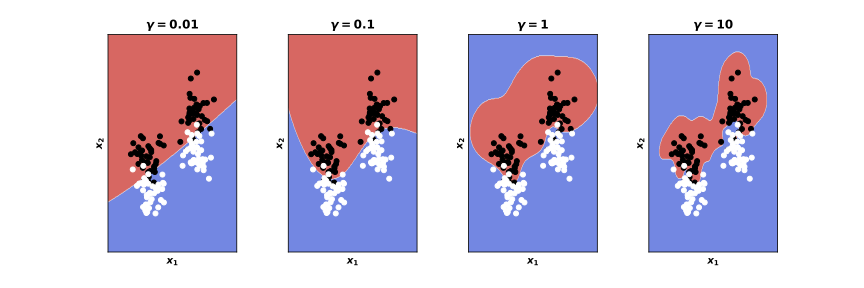
\includegraphics[width=0.80\textwidth]{../slides/diagrams/ml/bias-variance000.png}
\end{center}\begin{center}
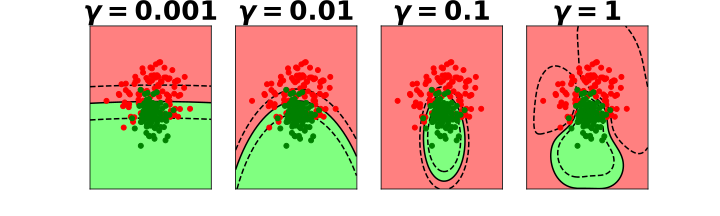
\includegraphics[width=0.80\textwidth]{../slides/diagrams/ml/bias-variance010.png}
\end{center}


\caption{In each figure the simpler model is on the left, and the more complex model is on the right. Each fit is done to a different version of the data set. The simpler model is more consistent in its errors (bias error), whereas the more complex model is varying in its errors (variance error).}
\label{bias-variance-errors}
\end{figure}

\hypertarget{double-descent}{%
\subsection{Double Descent}\label{double-descent}}


One of Breiman's ideas for improving predictive performance is known as
bagging \citep{Breiman:bagging96}. The idea is to train a number of
models on the data such that they overfit (high variance). Then average
the predictions of these models. The models are trained on different
bootstrap samples \citep{Efron:bootstrap79} and their predictions are
aggregated giving us the acronym, Bagging. By combining decision trees
with bagging, we recover random forests \citep{Breiman-forests01}.

Bias and variance can also be estimated through Professor Efron's
bootstrap \citep{Efron:bootstrap79}, and the traditional view has been
that there's a form of Goldilocks effect, where the best predictions are
given by the model that is `just right' for the amount of data
available. Not to simple, not too complex. The idea is that bias
decreases with increasing model complexity and variance increases with
increasing model complexity. Typically plots begin with the Mummy bear
on the left (too much bias) end with the Daddy bear on the right (too
much variance) and show a dip in the middle where the Baby bear (just)
right finds themselves.

The Daddy bear is typically positioned at the point where the model is
able to exactly interpolate the data. For a generalized linear model
\citep{McCullagh:gen_linear89}, this is the point at which the number of
parameters is equal to the number of data\footnote{Assuming we are
  ignoring parameters in the link function and the distribution
  function.}. But the modern empirical finding is that when we move
beyond Daddy bear, into the dark forest of the massively
overparameterized model we can achieve good generalization.

As \citet{Zhang:understanding17} starkly illustrated with their random
labels experiment, within the dark forest there are some terrible
places, big bad wolves of overfitting that will gobble up your model.
But as empirical evidence shows there is also a safe and hospitable
Grandma's house where these highly overparameterized models are safely
consumed. Fundamentally, it must be about the route you take through the
forest, and the precautions you take to ensure the wolf doesn't see
where you're going and beat you to the door.

There are two implications of this empirical result. Firstly, that there
is a great deal of new theory that needs to be developed. Secondly, that
theory is now obliged to conflate two aspects to modelling that we
generally like to keep separate: the model and the algorithm.

Classical statistical theory around predictive generalization focusses
specifically on the class of models that is being used for data fitting.
Historically, whether that theory follows a Fisher-aligned estimation
approach (see e.g.~\citet{Vapnik:book98}) or model-based Bayesian
approach (see e.g.~\citet{Ghahramani:probabilistic15}), neither is fully
equipped to deal with these new circumstances because, to continue our
rather tortured analogy, these theories provide us with a
characterization of the \emph{destination} of the algorithm, and seek to
ensure that we reach that destination. Modern machine learning requires
theories of the \emph{journey} and what our route through the forest
should be.

Crucially, the destination is always associated with 100\% accuracy on
the training set. An objective that is always achievable for the
overparameterized model.

Intuitively, it seems that a highly overparameterized model places
Grandma's house on the edge of the dark forest. Making it easily and
quickly accessible to the algorithm. The larger the model, the more
exposed Grandma's house becomes. Perhaps this is due to some form of
blessing of dimensionality brings Grandma's house closer to the edge of
the forest in a high dimensional setting. Really, we should think of
Grandma's house as a low dimensional manifold of destinations that are
safe. A path through the forest where the wolf of overfitting doesn't
venture. In the GLM case, we know already that when the number of
parameters matches the number of data there is precisely one location in
parameter space where accuracy on the training data is 100\%. Our
previous misunderstanding of generalization stemmed from the fact that
(seemingly) it is highly unlikely that this single point is a good place
to be from the perspective of generalization. Additionally, it is often
difficult to find. Finding the precise polynomial coefficients in a
least squares regression to exactly fit the basis to a small data set
such as the Olympic marathon data requires careful consideration of the
numerical properties and an orthogonalization of the design matrix
\citep{Lawson:least95}.

It seems that with a highly overparameterized model, these locations
become easier to find and they provide good generalization properties.
In machine learning this is known as the ``double descent phenomenon''
(see e.g.~\citet{Belkin:reconciling19}).

As Professor Efron points out, modern machine learning models are often
fitted using many millions of data points. The most extreme example of
late is known as GPT-3. This neural network model, known as a
Transformer, has in its largest form 175 billion parameters. The model
was trained on a data set containing 499 billion tokens (about 2
terabytes of text). Estimates suggest that the model costs around \$4.5
million dollars to train (see e.g.~\citet{Li:openai20}).

\hypertarget{empirical-effectiveness-of-deep-learning}{%
\subsection{Empirical Effectiveness of Deep
Learning}\label{empirical-effectiveness-of-deep-learning}}


The OpenAI model represents just a recent example from a wave of
\emph{deep} neural network models has proved highly performant across a
range of challenges that were previously seen as being beyond our
statistical modelling capabilities.

They stem from the courage of a group of researchers who saw that
methods were improving with increasing data and chose to collect and
label data sets of ever increasing size, in particular the ImageNet team
led by Fei-Fei Li \citep{Russakovsky-imagenet15} who collected a large
data set of images for object detection (currently 14 million images).
To make these neural network methods work on such large data sets new
implementations were required. By deploying neural network training
algorithms on graphics processing units (GPUs) breakthrough results were
achieved on these large data sets \citep{Krizhevsky:imagenet12}. Similar
capabilities have then been shown in the domains of face identification
\citep{Taigman:deepface14}, and speech recognition
\citep{Hinton:acoustic12}, translation \citep{Sutskever:sequence14} and
language modelling \citep{Radford:language19, Devlin:bert19}.

Impressive though these performances are, they are reliant on massive
data and enormous costs of training. Yet they can be seen through the
lens of regression, as outlined by Professor Efron in his paper. They
map from inputs to outputs. For language modelling, extensive use of
auto-regression allows for sequences to be generated.

\hypertarget{new-methods-required}{%
\section{New Methods Required}\label{new-methods-required}}


The challenges of big data emerged due to companies being able to
rapidly interconnect multiple sources of information. This leads to
challenges in storage, distributed processing and modeling. Google's
search engine was at the forefront of this revolution in data
processing. Google researchers were among the first to notice that some
tasks can be easily resolved with fairly simple models and very large
data sets \citep{Halevy:unreasonable09}. What we are now learning is
that many tasks can be solved with complex models and even bigger data
sets.

While GPT-3 does an impressive job on language generation, it can do so
because of the vast quantities of language data we have made available
to it. What happens if we take a more complex system, for which such
vast data is not available. Or, at least not available in the
homogeneous form that language data can be found. Let's take human
health.

Consider we take a holistic view of health and the many ways in which we
can become unhealthy, through genomic and environmental effects.
Firstly, let's remember that we don't have a full understanding, even on
all the operations in a single eukaryotic cell. Indeed, we don't even
understand all the mechanisms by which transcription and translation
occur in bacterial and archaeal cells. That is despite the wealth of
gene expression and protein data about these cells. Even if we were to
pull all this information together, would it be enough to develop that
understanding?

There are large quantities of data, but the complexity of the underlying
systems in these domains, even the terabytes of data we have today may
not be enough to determine the parameters of such complex models.

Machine learning involves taking data and combining it with a model in
order to make a prediction. The data consist of measurements recorded
about the world around us. A model consists of our assumptions about how
the data is likely to interrelate, typical assumptions include
smoothness. Our assumptions reflect some underlying belief about the
regularities of the universe that we expect to hold across a range of
data sets. \[
\text{data} + \text{model} \stackrel{\text{algorithm}}{\rightarrow}  \text{prediction}
\] The data and the model are combined in computation through an
algorithm. The etymology of the data indicates that it is given (data
comes from Latin \emph{dare}). In some cases, for example an approach
known as active learning, we have a choice as to how the data is gotten.
But our main control is over the model and the algorithm.

This is true for both statisticians and machine learning scientists.
Although there is a difference in the core motivating philosophy. The
mathematical statisticians were motivated by a desire to remove
subjectivity from the analysis, reducing the problem to rigorous
statistical proof. The statistician is nervous of the inductive biases
humans exhibit when drawing conclusions from data. Machine learning
scientists, on the other hand, sit closer to the artificial intelligence
community. Traditionally, they are inspired by human inductive biases to
develop algorithms that allow computers to emulate human performance on
tasks. In the past I've summarized the situation as

\begin{quote}
Statisticians want to turn humans into computers, machine learners want
to turn computers into humans. Neither is possible so we meet somewhere
in the middle.
\end{quote}

\hypertarget{traditional-model-algorithm-separation}{%
\subsection{Traditional Model-Algorithm
Separation}\label{traditional-model-algorithm-separation}}

Across both statistics and machine learning, the traditional view was
that the modeling assumptions are the key to making good predictions.
Those assumptions might include smoothness assumptions, or linearity
assumptions. In some domains we might also wish to incorporate some of
our mechanistic understanding of the data (see
e.g.~\citet{Alvarez:llfm13}). The paradigm of model-based machine
learning (\citet{Winn:mbml19}), builds on the idea that the aim of
machine learning is to describe one's views about the world as
accurately as possible within a model. The domain expert becomes the
model-designer. The process of algorithm design is then automated to as
great an extent as possible. This idea originates in the ground-breaking
work of the MRC Biostatistics Unit on BUGS that dates to 1997 (see
e.g.~Lunn-bugs09). It is no surprise that this notion has gained most
traction in the Bayesian community, because the probabilistic philosophy
promises the separation of modeling and inference. As long as the
probabilistic model we build is complex enough to capture the true
generating process, we can separate the process of model building and
probabilistic inference. Inference becomes turning the handle on the
machine. Unfortunately, the handle turning in Bayesian inference
involves high dimensional integrals and much of the work in this domain
has focused on developing new methods of inference based around either
sampling (see e.g.~\citet{Carpenter-stan17}) or deterministic
approximations (see e.g.~\citet{Tran-edward16}).

There are two principle challenges for model-based machine learning. The
first is the model design challenge, and the second is the algorithm
design challenge. The basic philosophy of the model-based approach is to
make it as easy as possible for experts to express their ideas in a
modeling language (typically probabilistic) and then automate as much as
possible the algorithmic process of fitting that model to data
(typically probabilistic inference).

The challenge of combining that model with the data, the algorithm
design challenge, is then the process of probabilistic inference.

The model is a mathematical abstraction of the regularities of the
universe that we believe underly the data as collected. If the model is
well-chosen, we will be able to interpolate the data and predict likely
values of future data points. If it is chosen badly our predictions will
be overconfident and wrong.


Deep learning methods conflate two
aspects that we used to try to keep distinct. The mathematical model
encodes our assumptions about the data. The algorithm is a set of
computational instructions that combine our modeling assumptions with
data to make predictions.

Much of the technical focus in machine learning is on algorithms. In
this document I want to retain a strong separation between the
\emph{model} and the \emph{algorithm}. The model is a mathematical
abstraction of the world that encapsulates our assumptions about the
data. Normally it will depend on one or more parameters which are
adaptable. The algorithm provides a procedure for adapting the model to
different contexts, often through the provision of a set of data that is
used for training the model.

Despite the different role of model and algorithm, the two concepts are
often conflated. This sometimes leads to a confused discussion. I was
recently asked ``Is it correct to remove the mean from the data before
you do principal component analysis.'' This question is about an
algorithmic procedure, but the correct answer depends on what modelling
assumption you are seeking to make when you are constructing your
principal component analysis. Principal component analysis was
originally proposed by a \emph{model} for data by
\citep{Hotelling:analysis33}. It is a latent variable model that was
directly inspired by work in the social sciences on factor analysis.
However, much of our discussion of PCA today focusses on PCA as an
algorithm. The algorithm for fitting the PCA model is to seek the
eigenvectors of the covariance matrix, and people often refer to this
algorithm as principal component analysis. However, that algorithm also
finds the linear directions of maximum variance in the data. Seeking
directions of maximum variance in the data was not the objective of
Hotelling, but it is related to a challenge posed by \citet{Pearson:01}
who sought a variant of regression that predicted symmetrically
regardless of which variable was considered to be the covariate and
which variable the response. Coincidentally the algorithm for this model
is also the eigenvector decomposition of the covariance matrix. However,
the underlying model is different. The difference becomes clear when you
begin to seek non-linear variants of principal component analysis.
Depending on your interpretation (finding directions of maximum variance
in the data or a latent variable model) the corresponding algorithm
differs. For the Pearson model a valid non-linearization is kernel PCA
\citep{Scholkopf:nonlinear98}, but for the Hotelling model this
generalization doesn't make sense. A valid generalization of the
Hotelling model is provided by the Gaussian process latent variable
model \citep{Lawrence:pnpca05}. This confusion is often unhelpful, so
for the moment we will leave algorithmic considerations to one side and
focus \emph{only} on the model.

\hypertarget{is-my-model-useful}{%
\subsection{Is my Model Useful?}\label{is-my-model-useful}}


In the first half of the 20th Century, the Bayesian approach was termed
\emph{inverse probability}. Fisher disliked the subjectivist nature of
the approach \citep{Aldrich-fisher08} and introduced the term
\emph{Bayesian} in 1950 to distinguish these probabilities from the
likelihood function \citep{Fisher-contributions50}. The word Bayesian
has connotations of a strand of religious thinking or a cult.\footnote{This
  was pointed out to me by Bernhard Schölkopf, who by recollection
  credited the observation to the philosopher David Corfield.} Whether
Fisher was fully aware of this when he coined the term we cannot know,
but there is a faith-based-tenet that at the heart of Bayesian ideas.

Many critics of the Bayesian approach ask where the Bayesian prior comes
from. But one might just as well ask, where does the likelihood come
from? Or where does the link function come from? All of these are
subjective modeling questions. The prior is not the problem. The
challenge is providing objective guarantees for our subjective model
choices. The classical Bayesian approach provides guarantees, but only
for the \(\mathcal{M}\)-closed domain \citep{Bernardo:bayesian94}, where
the \emph{true} model is one of the models under consideration. This is
the critical belief at the heart of the Church of Bayes: the doctrine of
model correctness.

The beauty of the Bayesian approach is that you don't have to have much
imagination. You work as hard as possible with your models of
probability distributions to represent the problem as best you
understand it, then you work as hard as possible to approximate the
posterior distributions of interest and estimate the marginal
likelihoods and any corresponding Bayes's factors. If we have faith in
the doctrine of model correctness, then we can pursue our modeling aims
without the shadows of doubt to disturb us.

Bayesian approaches have a lot in common with more traditional
regularization techniques. Ridge regression imposes L2 shrinkage on the
model's weights and has an interpretation as the maximum a posteriori
estimate of the Bayesian solution. For linear models the mathematics of
the two approaches is strikingly similar, and they both assume stages of
careful design of model/regularizer followed by either Bayesian
inference or optimization. The situation with the new wave of
overparameterized models is strikingly different.

\hypertarget{implicit-regularization}{%
\subsubsection{Implicit Regularization}\label{implicit-regularization}}

The new wave of overparameterized machine learning methods are
\emph{not} making this conceptual separation between the model and the
algorithm. Deep learning approaches are simple algorithmically, but
highly complex mathematically. By this I mean that it is relatively
simple to write code that creates algorithms for optimizing the neural
network models, particularly with the wide availability of automatic
differentiation software. But analyzing what these algorithms are doing
mathematically is much harder. Fortunately, insight can already be
gained by considering overparameterized models in the \emph{linear}
paradigm.

These analyses consider `gradient flow' algorithms. A gradient flow is
an idealization of the optimization where the usual stochastic gradient
descent optimization \citep{Robbins:stoch51} is replaced with
differential equations representing the idealized trajectory of a
\emph{batch} gradient descent approach. Under these analyses, highly
overparameterized linear models can be shown to converge to the L2 norm
solution (see e.g.~\citet{Soudry-implicit18}). It seems that stacking
layers of networks also has interesting effects, because even when
\emph{linear} models are stacked analysis of the learning algorithm
indicates a tendency towards low rank linear solutions for the
parameters \citep{Arora-convergence19}. These regularization approaches
are known as \emph{implicit} regularization, because the regularization
is implicit in the optimizer rather than explicitly declared by the
model-designer. These theoretical insights have also proven useful in
practice. \citet{Arora-implicit19} show state-of-the-art performance for
matrix factorization through exploiting implicit regularization in the
domain of matrix factorization.

Studying the implicit regularization of these modern overparameterized
machine learning methods is likely to prove a fruitful avenue for
theoretical investigation that will deliver deeper understanding of how
we can design traditional statistical models. But the conflation of
model and algorithm can make it hard to unpick what design choices are
influencing which aspects of the model.

While I've motivated much of this paper through the lens of happenstance
data. But the training sets that are used with these deep learning
models have striking similarities to classical data acquisition. The
deep learning revolution is really a revolution of ambition in the scale
of data which we are collecting. The data set which drove this paradigm
shift in data collection was ImageNet (see
e.g.~\citet{Russakovsky-imagenet15}). It was only with the millions of
labeled images available in the data that Fei-Fei Li's team assembled
that these highly overparameterized models were able to significantly
differentiate themselves from traditional approaches
\citep{Krizhevsky:imagenet12}. Collection of such massive data is
statistical design on a previously unprecedented scale requiring massive
human effort for labeling. That doesn't sit well with the notion of
happenstance data, which by its nature is accumulating fast and is only
lightly curated if at all. So, while acknowledging the importance and
benefits of implicit regularization we will revert to the conceptual
separation between model and algorithm as we consider what approaches
might be useful for this new data landscape.

\hypertarget{reviewing-the-traditional-paradigm}{%
\subsection{Reviewing the Traditional
Paradigm}\label{reviewing-the-traditional-paradigm}}

The modern Bayesian has a suite of different software available to make
it easier for her to design models and perform inference in the
resulting design. Given this extra time, it might depress her to reflect
on the fact that the entire premise of the approach is mistaken unless
you are in the \(\mathcal{M}\)-closed domain. So, when do we fall
outside this important domain? According to \citet{Box:science76}, all
the time.

\begin{quote}
All models are wrong, but some are useful
\end{quote}

Box's important quote has become worn by overuse (like a favorite
sweater). Indeed, I most often see it quoted at the beginning of a talk
in a way that confuses correlation with causality. Presentations proceed
in the following way. (1) Here is my model. (2) It is wrong. (3) Here is
George Box's quote. (4) My model is wrong, but it might be useful.
Sometimes I feel at stage (4) a confusion about the arrow of causality
occurs, it feels to me that people are almost saying ``\emph{Because} my
model is wrong it \emph{might} be useful.''

Perhaps we should be more focusing on the quote from the same
paper\footnote{This quote was first highlighted to me by Richard D.
  Wilkinson.}

\begin{quote}
the scientist must be alert to what is importantly wrong. It is
inappropriate to be concerned about mice when there are tigers abroad.

\citet{Box:science76}
\end{quote}

Let's have a think about where the tigers might be in the domain of big
data. To consider this, let's first see what we can write down about our
data that isn't implicitly wrong. If we are interested in multivariate
data, we could first write down our data as a \emph{design matrix} \[
\text{data} = \mathbf{\dataMatrix} \in \Re^{\numData\times \dataDim}.
\] Here we are assuming we have \(\numData\) data points and
\(\dataDim\) features. As soon as we write down our data in this form it
invites particular assumptions about the data that may have been valid
in the 1930s, when there was more focus on survey data. Experimental
designs stipulated a table of data with a specific set of hypotheses in
mind. The data naturally sat in a matrix.

The first thing that I was taught about probabilistic modeling was
i.i.d. noise. And as soon as we see a matrix of data, I believe it is
second nature for most of us to start writing down factorization
assumptions. In particular, an independence assumption across the
\(\numData\) data points, giving the likelihood function. \begin{align*}
p(\dataMatrix|\parameterVector) = \prod_{i=1}^\numData p(\dataVector_{i, :} | \boldsymbol{\theta}).
\end{align*} This factorization gives both practical and theoretical
advantages. It allows us to show that by optimizing the likelihood
function, we are minimizing a sample-based approximation to a
Kullback-Leibler divergence between our model and the true data
generating density (see e.g.~\citet{Wasserman:all03}). \begin{align*}
\log p(\dataMatrix|\parameterVector) =& \sum_{i=1}^\numData \log p(\dataVector_{i, :} | \boldsymbol{\theta}) + \text{const}
\approx & \int \Pr(\dataMatrix) \log \frac{p(\dataMatrix|\parameterVector)}{\Pr(\dataMatrix)}
\end{align*} where \(\Pr(\dataMatrix)\) is the true data generating
distribution.

From pragmatist's perspective, the assumption allows us to make
predictions about new data points given a parameter vector that is
derived from the training data. If the uncertainty in the system is
truly independent between different data observations, then the
information about the data is entirely stored in our model parameters,
\(\parameterVector\).

Much of classical statistics focusses on encouraging the data to conform
to this independence assumption, for example through randomizing the
design to distribute the influence of confounders and through selection
of appropriate covariates. Or to methodologies that analyze the model
fit to verify the validity of these assumptions, for example residual
analysis.

From a Bayesian perspective, this assumption \emph{is} only an
assumption about the nature of the residuals. It is \emph{not} a model
of the process of interest. The philosophical separation of aleatory
uncertainty and epistemic uncertainty occurs here. Probability is being
used only to deal with the aleatory uncertainty.

In the world of happenstance data, there is insufficient influence from
the model-designer on the way that the data is collected to rely on
randomization. We find ourselves needing to explicitly model
relationships between confounders. This requires us to be more
imaginative about our probabilistic models than pure independence
assumptions.

An additional challenge arising from this independence assumption is the
domain where the number of data features, \(\dataDim\), is larger than
the number of data points, \(\numData<<\dataDim\), the so called `large
\(\dataDim\), small \(\numData\)' domain. Classical methodologies fail
in this domain because the parameters are poorly determined.

\hypertarget{getting-rid-of-datadim}{%
\subsection{\texorpdfstring{Getting Rid of
\(\dataDim\)}{Getting Rid of \textbackslash dataDim}}\label{getting-rid-of-datadim}}

Despite the advantages of the classical statistical paradigm, I believe
it has lured us into a trap. The trap is that \(\dataDim\) exists. That
there is a particular dimensionality associated with the features, or
covariates, we associate with a typical response variable. As I think
about happenstance data, I've increasingly become to believe that
\(\dataDim\) doesn't really exist. It is a convenience for us. Or, at
least if it does exist, it is not fixed in dimension, it varies, just
like the number of data.

In programming language parlance, we treat \(\dataDim\) as a `static
variable'. One which stays the same size for the lifetime of the model.
We are prepared to accept that \(\numData\) will change, we will be
expected to make out of sample predictions, but we don't accept that we
might need to make `out of response-variable' predictions or
`out-of-covariate' predictions.

So, below, I intend to conflate \(\numData\) and \(\dataDim\). Rather
than considering a design matrix, \(\dataMatrix\), I'd like us to think
about a vector, \(\dataVector\), where each element of the vector arises
from a particular data-point but it could contain one of a number of
features from that data-point. The data moves from being a table, to a
vector of data snippets. Each element of the vector potentially coming
from a different subject and possibly encoding a different aspect of
that subject.

Now that we've decided we'll consider the data in a vector (if do you
have a design matrix, just stack the columns of the design matrix one on
top of another to form the vector), let's also drop the independence
assumption. Independence assumptions are very useful, and we will return
to them later. But for the moment let's assume it is not the first thing
we should write down.

\hypertarget{a-motivating-big-data-example}{%
\section{A Motivating Example}\label{a-motivating-big-data-example}}


To motivate the movement from matrix to vector, we'll consider the type
of challenge that might arise in today's era of happenstance data.
Mathematical statisticians worked with tables of data that they'd
carefully collected, often with the specific purpose of answering a
particular question. The decided at experiment \emph{design} time what
was to be measured \(\numData\). We continue to do this today; we even
use statistical power calculations to decide how many subjects we need
in our data sample.

Our motivation will be personalized health: what we can learn about
patients' state of health and when should we suggest interventions?

In the big data era, we are not only interested in what data we might
collect for answering a specific question (although this data remains
important) but we are also interested in existing data that might be
assimilated to improve our understanding of an individual's health. When
we imagine systems that can monitor our individual health status, we
should not be restricted to the type of data that might be stored in a
doctor's office or a hospital data base. We can even argue that that
hospital data focusses on sickness rather than health, giving us an
incomplete picture.

In the modern world of happenstance data, we might like to build models
that incorporate, for example, an individual's exercise regime (for
example through websites such as Strava). We could also include
information about an individual's dietary habits extracted from loyalty
card information like the Nectar card. If we were monitoring potential
degradation in health then we may also be interested in an individual's
social network activity (Twitter, Facebook, SnapChat). Even musical
tastes may feed into our overall picture of the patient's well-being
through music services like Spotify.

For a full perspective on a patient's health, this data needs to be
combined with more traditional sources like phenotype and genotype
information. For example, high resolution scans of the genome provide a
detailed characterization of genotype. Large-scale gene-expression
measurements, give high resolution understanding of phenotype at the
cellular level. Imaging domains can contain X-rays scans, MRIs or
pathologists' samples. Doctor's notes, both free-form notes and those
that encode diagnosis through emerging EHR/EMR coding standards such as
the WHO's International Classification of Diseases (ICD-11, see
\citet{WHO-icd20}). And also, the results of clinical tests, such as
cholesterol levels. To provide a full picture of health status all this
information needs to be assimilated.

In a traditional model, we might encode each piece of information as
another element on a feature vector: in other words, each data snippet
mentioned contributes to increasing \(\dataDim\). However, for most
patients, most of the information above will be missing. We obtain only
snippets of information about music tastes and social media habits
alongside the occasional clinical measurement. Missing data is often
discussed, but not at the scale we are considering here. In a classical
analysis we might consider 30\% missingness to be a big number. In this
new scenario of data snippets almost all the data is missing almost all
the time. A typical amount of missingness might be 99.9\%. The data
snippet domain is one which we might refer to as \emph{massively missing
data}. A situation where a missing value becomes the norm and a data
observation is the exception.

Alongside the patchy nature of these data snippets, another challenge
would be how they arrive. This happenstance data is constantly evolving.
In computer systems terminology it is referred to as streaming data. The
table form of the design matrix is a consequence of active surveillance
of the population. When acquiring data passively it updates haphazardly.

Our model may need to update because patient 2,342 has just had the
results of a blood test logged, or because patient 28,344,219 has just
been for a run or because patient 12,012,345 just listened to a Leonard
Cohen track or because patient 12,182 just gave birth.

For applications like the personalized health monitoring system
described above, we need a model that will give well calibrated
predictions from the first day of it being brought online, and
throughout its operational life. If the model is complex enough to
represent the full spectrum of possible human ailments, then when the
model is first brought on stream, it is unlikely to have sufficient data
to determine the parameters. In the standard modeling framework, we are
faced with the bias-variance dilemma \citep{Geman:bias92}. If the model
is complex enough to represent the underlying data structure, the
parameters will be badly determined for small, or badly designed data
sets, and the model will exhibit a large error due to variance. We are
still learning how the deep learning frameworks provide a route out of
this dilemma. A part of the story is their overparameterization. But
what is the formalism by which we can incorporate more information about
each individual patient within these highly parameterized models?

A major challenge in the domain we've described is to build a model that
is complex enough to represent the diversity of human health outcomes.
For streaming data this necessarily means that some (or most) of those
parameters will be badly determined. This is reminiscent of the
overparameterized deep learning models.

\hypertarget{uncertainty-in-parameters}{%
\subsection{Uncertainty in
Parameters}\label{uncertainty-in-parameters}}


When parameters are badly determined, we expect high variance. So, small
fluctuations in the data set should lead to larger fluctuations in
prediction. One approach to this problem is to build models in which the
parameters are well determined. For the independence across data points
case, this involves having many observations (large \(\numData\))
relative to the number of parameters (which often scales with
\(\dataDim\)). This motivates the issues of the large \(\dataDim\) small
\(\numData\) domain, where the conditions are reversed. Of course, from
a modelling perspective this issue is trivially solved by assuming
independence across the \(\dataDim\) data dimensions and allowing the
parameters to scale with the number of data \(\numData\). This is a
characteristic exhibited, for example by the Gaussian process latent
variable model \citep{Lawrence:pnpca05} which in standard form assumes
independence across \(\dataDim\) for high dimensional data and
associates each data point with a latent variable that is treated as a
parameter. In \citep{Lawrence:unifying12} I argued that the successful
class of \emph{spectral} approaches to dimensionality reduction (e.g.
LLE \citet{Roweis:lle00} and maximum variance unfolding
\citet{Weinberger:learning04}, which are widely applied in the large
\(\dataDim\) small \(\numData\) domain, also have a probabilistic
interpretation where the underlying likelihood factorizes across data
dimensions. For these models, dimensionality becomes a blessing rather
than a curse. It's a neat trick, but it still doesn't solve the
fundamental problem. What happens when \(\numData \approx \dataDim\)?
Neither factorization leads to well determined parameters.

\hypertarget{massively-missing-data}{%
\subsection{Massively Missing Data}\label{massively-missing-data}}

I'm going to argue that the separation of the data into features and
data points is a distraction for happenstance data. It stems from
mathematical statistics when the intention was to make a strong
scientific claim based on numbers take from a \emph{table} of data. A
table naturally lends itself towards a matrix form. In these data a
statistical design normally involved measuring a fixed number of
\emph{features} for a perhaps variable number of \emph{items}. The
objective is to find sufficient number of items so that you can make
strong claims about which features are important. For example, does
smoking correlate with lung cancer? This explains the desire to write
down the data as a matrix \(\dataMatrix\). I think this view of data,
while historically important and still of great utility today, is
restrictive when considering modern big data problems.

The modern data analysis challenge is very different. We receive
streaming data of varying provenance. If each number we receive is given
by an observation \(\dataScalar_i\), where \(\dataScalar_i\) could be in
the natural numbers, the real numbers, binary or in any processable
form, then \(\dataScalar_{17}\) might be the price of a return rail fair
from Sheffield to Oxford on 6th February 2014, whilst
\(\dataScalar_{29}\) might be the number of people on the 8:20 train
that day, but \(\dataScalar_{72,394}\) could be the temperature of the
Atlantic ocean on 23rd August 2056 at a point on the Arctic circle
midway between Greenland and Norway. When we see data in this form, we
realize that most of the time we are missing most of the data. This
leads to the idea of \emph{massive missing data}. Contrast this
situation with that traditionally faced in missing data where a table of
values, \(\dataMatrix\), might have 10\%-50\% of the measurements
missing, perhaps due to problems in data collection. I'd argue that if
we are to model complex processes (such as the brain, or the cell, or
human health) then almost all the data is missing.

\begin{figure}[htb]
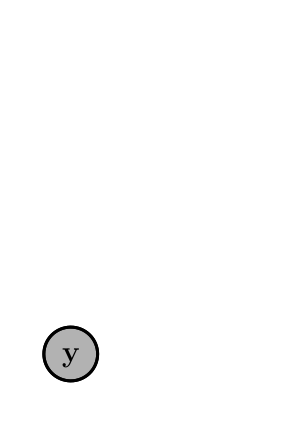
\includegraphics[width=0.30\textwidth]{../slides/diagrams/ml/y-only-graph.pdf}


\caption{The most general graphical model. It makes no assumptions about conditional probability relationships between variables in the vector $\dataVector$. It represents the unconstrained probability distribution $p(\dataVector)$.}
\label{y-only-graph}
\end{figure}

Figure \ref{y-only-graph} gives a graphical representation of a model
that's not wrong, just not useful. I like graphical representations of
probabilistic models and this is my favorite graph. It is the simplest
graph but also the most general model. It says that all the data in our
vector \(\dataVector\) is governed by an unspecified probability
disribution \(p(\dataVector)\).

Graphical models normally express the conditional independence
relationships in the data, with this graph we are not a priori
considering any such relationships. This is the most general model (it
includes all factorized models as special cases). It is not wrong, but
since it doesn't suggest what the next steps are or give us any handles
on the problem it is also not useful.

\hypertarget{big-data-consistency}{%
\subsection{Big Data Consistency}\label{big-data-consistency}}


This is the nature of modern streaming data, what has been called big
data, although in the UK it looks like that term will gain a more
diffuse meaning now that the government has associated a putative 189
billion pounds of funding to it. But the characteristic of massive
missing data is particularly obvious when we look at clinical domains.
EMIS, a Yorkshire based provider of software to General Practitioners,
has 39 million patient records. When we consider clinical measurements,
we need to build models that not only take into account all current
clinical tests, but all tests that will be invented in the future. This
leads to the idea of massive missing data. The classical statistical
table of data is merely the special case where someone has filled in a
block of information.

To deal with massively missing data we need to think about the
\emph{Kolmogorov consistency} of a process. Let me introduce Kolmogorov
consistency by way of an example heard from Tony O'Hagan, but one that
he credits originally to Michael Goldstein. Imagine you are on jury
duty. You are asked to adjudicate on the guilt or innocence of Lord
Safebury, and you are going to base your judgement on a model that is
weighing all the evidence. You are just about to pronounce your decision
when a maid comes running in and shouts ``He didn't do it! He didn't do
it!''. The maid wasn't on the witness list and isn't accounted for in
your model. How does this effect your inference? The pragmatists answer
might be: ``not at all, because the maid wasn't in the model.'' But in
the interests of justice we might want to include this information in
our inference process. If, as a result of the maid's entry, we now think
it is less likely that Lord Safebury committed the crime, then
necessarily every time that the (unannounced) maid doesn't enter the
room we have to assume that it is more likely that Safebury committed
the crime (to ensure that the conditional probability of guilt given the
maid's evidence normalizes. But we didn't know about the maid, so how
can we account for this? Further, how can we account for all possible
other surprise evidence, from the announced butlers, gardeners,
chauffeurs and footmen? Kolmogorov consistency says that the net effect
of marginalizing for all these potential bits of new information is
null. It is a particular property of the model. Making it (only
slightly) more formal, we can consider Kolmogorov consistency as a
marginalization property of the model. We take the \(\numData\)
dimensional vector, \(\dataVector\), to be an (indexed) vector of all
our instantiated observations of the world that we have \emph{at the
current time}. Then we take the \(\numData^*\) dimensional vector,
\(\dataVector^*\) to be the observations of the world that we are
\emph{yet to see}. From the sum rule of probability we have
\begin{align*} 
p(\dataVector|\numData^*) = \int p(\dataVector, \dataVector^*) \text{d}\dataVector^*,
\end{align*} where the dependence of the marginal distribution for
\(\dataVector\) aries from the fact that we are forming an
\(\numData^*\) dimensional integral over \(\dataVector^*\). If our
distribution is Kolmogorov consistent, then we know that the
distribution over \(\dataVector\) is \emph{independent} of the value of
\(\numData^*\). So, in other words
\(p(\dataVector|\numData*)=p(\dataVector)\). Kolmogorov consistency says
that the form of \(p(\dataVector)\) remains the same \emph{regardless}
of the number of observations of the world that are yet to come.

\hypertarget{parametric-models}{%
\subsection{Parametric Models}\label{parametric-models}}

We can achieve Kolomogrov consistency almost trivially in a parametric
model if we assume that the probability distribution is independent
given the parameters. Then the property of being closed under
marginalization is trivially satisfied through the independence,
\begin{align*}
p(\dataVector, \dataVector^*) = \int\prod_{i=1}^\numData p(\dataScalar_{i} |
\boldsymbol{\theta})\prod_{i=1}^{\numData^*}p(\dataScalar^*_i|\boldsymbol{\theta})
p(\paramVector) \text{d}\paramVector,
\end{align*} which allows us to marginalize for all future data leaving
a joint distribution which isn't dependent on \(\numData^*\) because
each future data point can be marginalized independently. \begin{align*}
p(\dataVector) = \int \prod_{i=1}^\numData
p(\dataScalar_{i} |
\boldsymbol{\theta})\prod_{i=1}^{\numData^*} \int
p(\dataScalar^*_i|\boldsymbol{\theta})
\text{d}\dataScalar^*_i p(\paramVector).
\text{d}\paramVector
\end{align*} But, as we've already argued, this involves an assumption
that is often flawed in practice. It is unlikely that, in a complex
model, we will be able to determine the parameter vector well enough,
given limited data, for us to truly believe that all the information
about the training data that is required for predicting the test data
could be passed through a fixed length parameter vector. This is what
this independence assumption implies. If we consider that the model will
also be acquiring new data at run time, then there is the question of
hot to update the parameter vector in a consistent manner, accounting
for new information, e.g.~new clinical results in the case of
personalized health.

Conversely, a general assumption about independence across
\emph{features} would lead to models which \emph{don't} exhibit
\emph{Komlogorov consistency}. In these models the dimensionality of the
test data, \(\dataVector^*\), denoted by \(\numData^*\) would have to be
fixed and each \(\dataScalar^*_i\) would require marginalization. So,
the nature of the test data would need to be known at model
\emph{design} time.

\hypertarget{parametric-bottleneck}{%
\subsection{Parametric Bottleneck}\label{parametric-bottleneck}}


In practice Bayesian methods suggest placing a prior over
\(\boldsymbol{\theta}\) and using the posterior,
\(p(\boldsymbol{\theta}|\dataVector)\) for making predictions.
\begin{align*} p(\dataVector^*|\dataVector) = \int \prod_i
p(\dataScalar_i^* |
\boldsymbol{\theta})p(\boldsymbol{\theta}|\dataVector)\text{d}\boldsymbol{\theta}.
\end{align*} We have a model that obeys Kolmogorov consistency, and is
sophisticated enough to represent the behavior of a very comlex dataset,
it may well require a large number of parameters, just like those deep
learning models. One way of seeing the requirement for a large number of
parameters is to look at how we are storing information from the
training data to pass to the test data. The sum of all our knowledge
about the training data is stored in the conditional distribution of the
parameters given the training data, the Bayesian \emph{posterior}
distribution, \(p(\paramVector | \dataVector).\)

A key design-time problem is the \emph{parametric bottleneck}. If we
choose the number of parameters at design time, but the system turns out
to be more complicated that we expected, we need to design a new model
to deal with this complexity. The communication between the training
data and the test data is like an information channel. This TT channel
has a bandwidth that is restricted by our choice of the dimensionality
of \(\boldsymbol{\theta}\) at \emph{design} time. This seems foolish. It
is the bonds of this constraint that deep learning models are breaking
by being so over-parameterized.

To deal with this challenge in a probabilistic model, we should allow
for a communication channel that is very large, or potentially infinite.
In mathematical terms this implies we should look at nonparametric
approaches.

If highly overparameterized models are the solution for deep learning,
then extending to nonparametric could be the solution to retaining the
necessary sense of indeterminedness that is required to cope with very
complex systems when we have seen relatively little data.

\hypertarget{the-nonparametric-challenge}{%
\subsection{The Nonparametric
Challenge}\label{the-nonparametric-challenge}}


We have argued that we want models that are unconstrained, at design
time, by a fixed bandwidth for the communication between the training
data, \(\dataVector\), and the test data, \(\dataVector^*\) and that the
answer is to be nonparametric. By nonparametric we are proposing using
classes of models for which the conditional distribution,
\(p(\dataVector^*|\dataVector)\) is not decomposable into the
expectation of \(p(\dataVector^*|\paramVector)\) under the posterior
distribution of the parameters, \(p(\paramVector|\dataVector)\) for any
fixed length parameter vector \(\paramVector\). We don't want to impose
such a strong constraint on our model at \emph{design time}. Our model
may be required to be operational for many years and the true complexity
of the system being modeled may not even be well understood at
\emph{design time}. We must turn to paradigms that allow us to be
adaptable at \emph{run time}. Nonparametrics provides just such a
paradigm, because the effect parameter vector increases in size as we
observe more data. This seems ideal, but it also presents a problem.

Human beings, despite are large, interconnected brains, only have finite
storage. It is estimated that we have between 100 and 1000 trillion
synapses in our brains. Similar for digital computers, even the GPT-3
model is restricted to 175 billion parameters. So, we need to assume
that we can only store a finite number of things about the data
\(\dataVector\). This seems to push us back towards nonparametric
models. Here, though, we choose to go a different way. We choose to
introduce a set of auxiliary variables, \(\inducingVector\), which are
\(\numInducing\) in length. Rather than representing the nonparametric
density directly, we choose to focus on storing information about
\(\inducingVector\). By storing information about these variables,
rather than storing all the data \(\dataVector\) we hope to get around
this problem. In order for us to be nonparametric about our predictions
for \(\dataVector*\) we must condition on all the data, \(\dataVector\).
We can't any longer store an intermediate distribution to represent our
sum knowlege, \(p(\paramVector|\dataVector)\). Such an intermediate
distribution is a finite dimensional object, and nonparametrics implies
that we cannot store all the information in a finite dimensional
distribution. This presents a problem for real systems in practice. We
are now faced with a compromise; how can we have a distribution which is
flexible enough to respond at \emph{run time} to unforeseen complexity
in the training data? Yet, simultaneously doesn't require unbounded
storage to retain all the information in the training data. We will now
introduce a perspective on variational inference that will allow us to
retain the advantages of both worlds. We will construct a parametric
approximation to the true nonparametric conditional distribution. But,
importantly, whilst this parametric approximation will suffer from the
constraints on the bandwidth of the TT channel that drove us to
nonparametric models in the first place, we will be able to change the
number of parameters at \emph{run time} not simply at design time.

\hypertarget{the-multivariate-gaussian-closure-under-marginalization}{%
\subsubsection{The Multivariate Gaussian: Closure Under
Marginalization}\label{the-multivariate-gaussian-closure-under-marginalization}}


Being closed under marginalization is a remarkable property of our old
friend the multivariate Gaussian distribution (old friends often have
remarkable properties that we often take for granted, I think this is
particularly true for the multivariate Gaussian). In particular, if we
consider a joint distribution across \(p(\dataVector, \dataVector^*)\),
then the covariance matrix of the marginal distribution for the subset
of variables, \(\dataVector\), is unaffected by the length of
\(\dataVector^*\). Taking this to its logical conclusion, if the length
of the data, \(\dataVector\), is \(\numData=2\). Then that implies that
the covariance between \(\dataVector\), as defined by \(\kernelMatrix\),
is only a \(2\times 2\) matrix, and it can only depend on the indices of
the two data points in \(\dataVector\). Since this covariance matrix
must remain the same for any two values \emph{regardless} of the length
of \(\dataVector\) and \(\dataVector^*\) then the value of the elements
of this covariance must depend only on the two indices associated with
\(\dataVector\).

Since the covariance matrix is specified pairwise, this implies that the
covariance matrix must be dependent only on the index of the two
observations \(\dataScalar_i\) and \(\dataScalar_j\) for which the
covariance is being computed. In general, we can also think of this
index as being infinite: it could be a spatial or temporal location.
\begin{align*} 
p(\dataVector) = \int p(\dataVector, \dataVector^*)
\text{d}\dataVector^*=
\frac{\exp\left(\begin{bmatrix}\dataVector \\
\dataVector^*\end{bmatrix}^\top\begin{bmatrix}\kernelMatrix &
\kernelMatrix_* \\ \kernelMatrix_*^\top &
\kernelMatrix_{**}\end{bmatrix}^{-1} \begin{bmatrix}\dataVector \\
\dataVector^*\end{bmatrix}\right)}{\int
\exp\left(\begin{bmatrix}\dataVector \\
\dataVector^*\end{bmatrix}^\top\begin{bmatrix}\kernelMatrix &
\kernelMatrix_* \\ \kernelMatrix_*^\top &
\kernelMatrix_{**}\end{bmatrix}^{-1} \begin{bmatrix}\dataVector \\
\dataVector^*\end{bmatrix}\right) \text{d}\dataVector
\text{d}\dataVector^*} = \mathcal{N}(\mathbf{0} |\kernelMatrix),
\end{align*} where each \(\dataScalar_i\) is now defined across the real
line, and the dimensionality of \(\dataVector*\) is irrelevant.
Prediction consists of conditioning the joint density on
\(\dataVector^*\). So, for any new value of \(\dataVector^*\), given its
index we compute \(p(\dataVector^* | \dataVector)\).

\hypertarget{making-parameters-nonparametric}{%
\subsection{Making Parameters
Nonparametric}\label{making-parameters-nonparametric}}


We will start by introducing a set of variables, \(\inducingVector\),
that are finite dimensional. These variables will eventually be used to
communicate information between the training and test data, i.e.~across
the TT channel. \[
p(\dataVector^*|\dataVector) = \int p(\dataVector^*|\inducingVector) q(\inducingVector|\dataVector) \text{d}\inducingVector
\] where we have introduced a distribution over \(\inducingVector\),
\(q(\inducingVector|\dataVector)\) which is not necessarily the true
posterior distribution, indeed we typically derive it through a variational approximation (see e.g.~\citet{Titsias:variational09}).

\begin{figure}[htb]
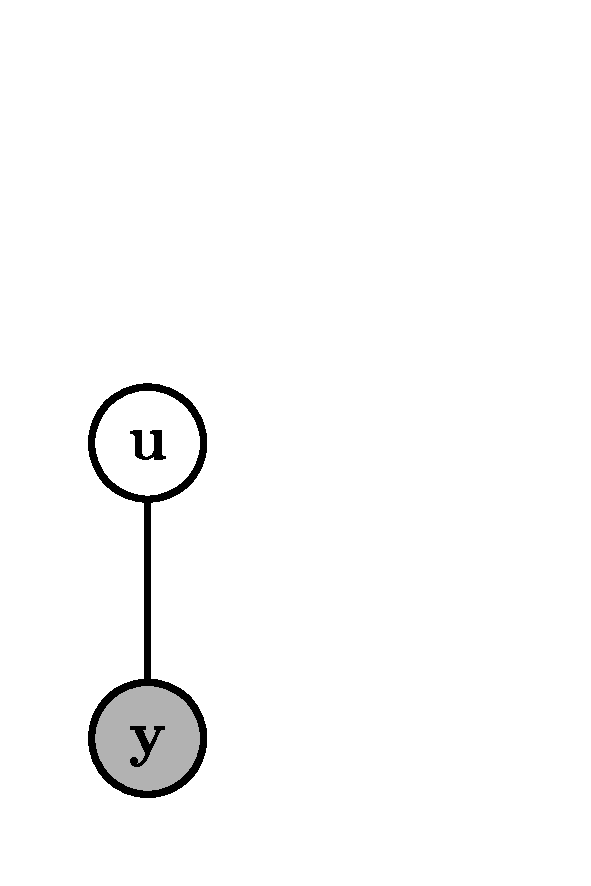
\includegraphics[width=0.3\textwidth]{../slides/diagrams/ml/u-to-y.pdf}


\caption{Augmenting the variable space with a set of latent \emph{inducing vectors}. The graphical model represents the factorization of the distribution into the form $\int p(\dataVector|\inducingVector)p(\inducingVector)\text{d}\inducingVector$}
\label{u-to-y}
\end{figure}

In Figure \ref{u-to-y} we have augmented our simple graphical model
augmented with a vector \(\inducingVector\) which we refer to as
inducing variables. Note that the model is still totally general because
\(p(\dataVector, \inducingVector)\) is an augmented variable model and
the original \(p(\dataVector)\) is easily recovered by simple
marginalization of \(\inducingVector\). So we haven't yet made any
assumptions about our data, our model is still correct, but useless.

The model we've introduced now looks somewhat like the parametric model
we argued against in the previous section, \[
p(\dataVector^* | \dataVector)=\int
p(\dataVector^*|\parameterVector)p(\parameterVector|\dataVector)\text{d}\parameterVector.
\] What's going on here? Is there going to be some kind of
parametric/nonparametric 3 card trick where with sleight of hand we are
trying to introduce a parametric model? Well clearly not, because I've
just given the game away. But I believe there are some important
differences to the traditional approach for parameterizing a model.
Philosophically, our variables \(\inducingVector\) are variables that
augment the model. We have not yet made any assumptions by introducing
them. Normally, parameterization of the model instantiates assumptions,
but this is not happening here. In particular note that we have
\emph{not} assumed that the training data factorize given the inducing
variables. Secondly, have not specified the dimensionality of
\(\inducingVector\) (i.e.~the size of the TT channel) at \emph{design}
time. We are going to allow it to change at \emph{run} time. We will do
this by ensuring that the inducing variables also obey Kolmogorov
consistency. In particular we require that If we build a joint density
as follows: \begin{align*} 
p(\dataVector, \inducingVector|\numInducing^*,
\numData^*) = \int p(\dataVector^*, \dataVector,
\inducingVector^*, \inducingVector) \text{d}\dataVector^*
\text{d}\inducingVector^*,
\end{align*} where \(\inducingVector\) are the inducing variables we
choose might choose to instantiate at any given time (of dimensionality
\(\numInducing\)) and \(\inducingVector^*\) is the \(\numInducing^*\)
dimensional pool of future inducing variables we have \emph{not yet}
chosen to instantiate (where \(\numInducing^*\) could be infinite). Our
new Kolmogorov consistency condition requires that \[
p(\dataVector, \inducingVector|\numInducing^*,\numData^*) = p(\dataVector, \inducingVector).
\] It doesn't need to be predetermined at \emph{design time} because we
allow for the presence of a (potentially infinite) number of inducing
variables \(\inducingVector^*\) that we may wish to \emph{later}
instantiate to improve the quality of our model. In other words, it is
very similar to the parametric approach, but now we have access to a
future pool of additional parameters, \(\inducingVector^*\) that we can
call upon to increase the bandwidth of the TT channel as appropriate. In
parametric modelling, calling upon such parameters has a significant
effect on the likelihood of the model, but here these variables are
auxiliary variables that will \emph{not} affect the likelihood of the
model. They merely effect our ability to approximate the true bandwidth
of the TT channel. The quality of this approximation can be varied at
run time. It is not necessary to specify it at design time. This gives
us the flexibility we need in terms of modeling, whilst keeping
computational complexity and memory demands manageable and appropriate
to the task at hand.

\begin{figure}[htb]
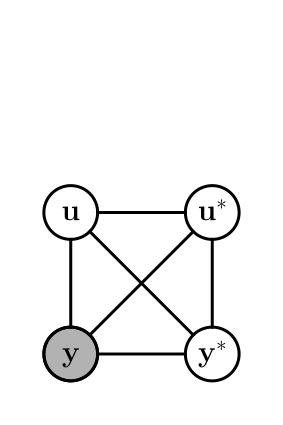
\includegraphics[width=0.30\textwidth]{../slides/diagrams/ml/u-to-y-ustar-to-y.pdf}


\caption{We can also augment the graphical model with data that is only seen at 'run time', or 'test data'. In this case we use the superscript of $*$ to indicate the test data. This graph represents the interaction between data we've seen, $\dataVector$, and data we've yet to see, $\dataVector^*$ as well as the augmented variables $\inducingVector$ and $\inducingVector$, $p(\dataVector) = \int p(\dataVector, \dataVector^*, \inducingVector, \inducingVector^*) \text{d}\dataVector^* \text{d}\inducingVector \text{d}\inducingVector^*$. As the fully connected graph implies we are making no assumptions about the data.}
\label{u-to-y-ustar-to-y}
\end{figure}

Adding in the test data and the inducing variables we have not yet
chosen to instantiate (Figure \ref{u-to-y-ustar-to-y}). Here we see that
we still haven't defined any structure in the graph, and therefore we
have not yet made any assumptions about our data. Not shown in the graph
is the additional assumption that whilst \(\dataVector\) has
\(\numData\) dimensions and \(\inducingVector\) has \(\numInducing\)
dimensions, \(\dataVector^*\) and \(\inducingVector^*\) are potentially
infinite dimensional.

\hypertarget{fundamental-variables}{%
\subsubsection{Fundamental Variables}\label{fundamental-variables}}

To focus our model further, we assume that we observe observations,
\(\dataVector\) that are derived from some underlying fundamental,
\(\mappingFunctionVector\), through simple factorized likelihoods. The
idea of the fundamental variables is that they are sufficient to
describe the world around us, but we might not be able to observe them
directly. In particular we might observe relatively simple corruptions
of the fundamental variables such as independent addition of noise, or
thresholding. We might observe something relative about two fundamental
variables. For example if we took \(\mappingFunction_{12,345}\) to be
the height of Tom Cruise and \(\mappingFunction_{23,789}\) to be the
height of Penelope Cruz then we might take for an observation a binary
value indicating the relative heights, so
\(\dataScalar_{72,394} = \mappingFunction_{12,345} < \mappingFunction_{23,789}\).
The fundamental variable is an artificial construct, but it can prove to
be a useful one. In particular we'd like to assume that the relationship
between our observations, \(\dataVector\) and the fundamental variables,
\(\mappingFunctionVector\) might factorize in some way. In the framework
we think of this relationship, given by
\(p(\dataVector|\inducingVector)\) as the \emph{likelihood}. We can
ensure that assuming the likelihood factorizes does not at all reduce
the generality of our model, by forcing the distribution over the
fundamentals, \(p(\mappingFunctionVector)\) to also be Kolmogorov
consistent. This ensures that in the case where the likelihood is fully
factorized over \(\numData\) the model is still general if we allow the
factors of the likelihood to be Dirac delta functions suggesing that
\(\dataScalar_i = \mappingFunction_i\). Since we haven't yet specified
any forms for the probability distributions this \emph{is} allowed and
therefore the formulation is still totally general. \[
p(\dataVector|\numData^*) = \int p(\dataVector|\mappingFunctionVector) p(\mappingFunctionVector, \mappingFunctionVector^*)\text{d}\mappingFunctionVector \text{d}\mappingFunctionVector^*
\] and since we enforce Kolmogorov consistency, we have \[
p(\dataVector|\numData^*) = p(\dataVector).
\]

\begin{figure}[htb]
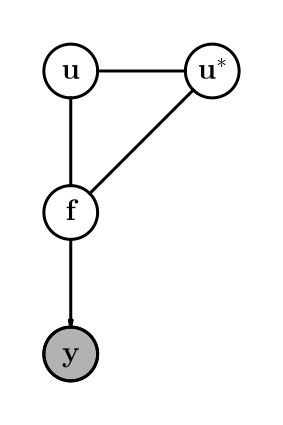
\includegraphics[width=0.30\textwidth]{../slides/diagrams/ml/u-to-f-to-y-ustar-to-f.pdf}


\caption{We introduce the fundamental variable $\mappingFunctionVector$ which sits between $\inducingVector$ and $\dataVector$.}
\label{u-to-f-to-y-ustar-to-f}
\end{figure}

Now we assume some form of factorization for our data observations,
\(\dataVector\), given the fundamental variables,
\(\mappingFunctionVector\), so that we have \[
p(\dataVector|\mappingFunctionVector) = \prod_{i} p(\dataVector^i| \mappingFunctionVector^i)
\] so that we have subsets of the data \(\dataVector^i\) which are
dependent on subsets of the fundamental variables, \(\mappingFunction\).
For simplicity of notation we will assume a factorization across the
entire data set, so each observation, \(\dataScalar_i\), has a single
underlying fundamental variable, \(\mappingFunction_i\), although more
complex factorizations are also possible and can be considered within
the analysis. \[
p(\dataVector|\mappingFunctionVector) = \prod_{i=1}^\numData p(\dataScalar_i|\mappingFunction_i)
\]

\begin{figure}[htb]
\includegraphics[width=0.30\textwidth]{../slides/diagrams/ml/u-to-f_i-to-y_i-ustar-to-f.pdf}


\caption{The relationship between $\mappingFunctionVector$ and $\dataVector$ is assumed to be factorized, which we indicate here using plate notation, $p(\dataVector) = \int \prod_{i=1}^\numData p(\dataScalar_i|\mappingFunction_i) p(\mappingFunctionVector | \inducingVector, \inducingVector^*) p(\inducingVector, \inducingVector^*)\text{d}\inducingVector \text{d}\inducingVector^*$.}
\label{u-to-f_i-to-y_i-ustar-to-f}
\end{figure}

We now decompose, without loss of generality, our joint distribution
over inducing variables and fundamentals into the following parts \[
p(\inducingVector, \mappingFunctionVector) = p(\mappingFunctionVector|\inducingVector)p(\inducingVector),
\] where we assume that we have marginalized
\(\mappingFunctionVector^*\) and \(\inducingVector^*\).



\begin{figure}[htb]
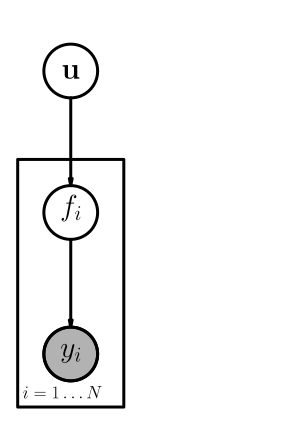
\includegraphics[width=0.30\textwidth]{../slides/diagrams/ml/u-to-f_i-to-y_i.pdf}


\caption{The model with future inducing points marginalized $p(\dataVector) = \int \prod_{i=1}^\numData p(\dataScalar_i|\mappingFunction_i) p(\mappingFunctionVector | \inducingVector) p(\inducingVector)\text{d}\inducingVector$.}
\label{u-to-f_i-to-y_i}
\end{figure}



\begin{figure}[htb]
\includegraphics[width=0.30\textwidth]{../slides/diagrams/ml/given-u-to-f_i-to-y_i.pdf}


\caption{The model conditioned on the inducing variables $p(\dataVector|\inducingVector, \inducingVector^*) = \int\prod_{i=1}^\numData p(\dataScalar_i|\mappingFunction_i) p(\mappingFunctionVector|\inducingVector, \inducingVector^*)\text{d}\mappingFunctionVector$.}
\label{given-u-to-f_i-to-y_i}
\end{figure}



\begin{figure}[htb]
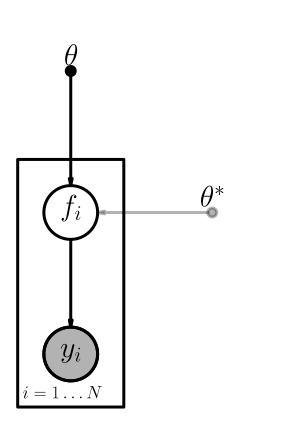
\includegraphics[width=0.30\textwidth]{../slides/diagrams/ml/given-theta-to-f_i-to-y_i.pdf}


\caption{The model as a classical parametric model with independence across data points indexed by $i$ that is conditional on parameters $\parameterVector$, $p(\dataVector|\parameterVector) = \int\prod_{i=1}^\numData p(\dataScalar_i|\mappingFunction_i) p(\mappingFunctionVector|\parameterVector)\text{d}\mappingFunctionVector$. The model is graphically the same as the nonparametric variant but here the dimension of $\parameterVector$ has to be fixed for Kolmogorov consistency, in the inducing vector variant the dimension of $\inducingVector$ can vary.}
\label{given-theta-to-f_i-to-y_i}
\end{figure}

\hypertarget{instantiating-the-model}{%
\subsection{Instantiating the Model}\label{instantiating-the-model}}

So far, we haven't made \emph{any} assumptions about the data in our
model, other than a factorization assumption between the fundamental
variables and the observations, \(\dataVector\). Even this assumption
does not affect the generality of the model decomposition, because in
the worst case the likelihood \(p(\dataVector|\mappingFunctionVector)\)
could be a Dirac \(\delta\) function, implying
\(\dataVector=\mappingFunctionVector\) and allowing us to include
complex interelations between \(\dataVector\) directly in
\(p(\mappingFunctionVector)\). We have specified that
\(p(\mappingFunctionVector, \inducingVector)\) should be Kolmogorov
consistent with \(\mappingFunctionVector^*\) and \(\inducingVector^*\)
being marginalized and we have argued that nonparametric models are
important in practice to ensure that all the information in our training
data can be passed to the test data.

For a model to be useful, we need to specify relationships between our
data variables. Of course, this is the point at which a model also
typically becomes wrong. At least if our model isn't correct, then it
should be a useful abstraction of the system.

\hypertarget{gaussian-processes}{%
\subsubsection{Gaussian Processes}\label{gaussian-processes}}

A flexible class of models that fulfils the constraints of being
non-parametric and Kolmogorov consistent is Gaussian processes. A
Gaussian process prior for our fundamental variables,
\(\mappingFunctionVector\) assumes that they are jointly Gaussian
distributed. Each data point, \(\mappingFunction_i\), is is jointly
distributed with each other data point \(\mappingFunction_j\) as a
multivariate Gaussian. The covariance of this Gaussian is a function of
the indices of the two data, in this case \(i\) and \(j\). But these
indices are not just restricted to discrete values. The index can be a
continuous value such as time, \(t\), or spatial location,
\(\inputVector\). The words index and indicate have a common etymology.
This is appropriate because the index indicates the provenance of the
data. In effect we have multivariate indices to account for the full
provenance, so that our observations of the world are given as a
function of, for example, the when, the where and the what. ``When'' is
given by time, ``where'' is given by spatial location and ``what'' is
given by a (potentially discrete) index indicating the further
provenance of the data. To define a joint Gaussian density, we need to
define the mean of the density and the covariance. Both this mean and
the covariance also need to be indexed by the when, the where and the
what.

\hypertarget{augmenting-with-inducing-variables-in-gaussian-processes}{%
\subsection{Augmenting with Inducing Variables in Gaussian
Processes}\label{augmenting-with-inducing-variables-in-gaussian-processes}}

To define our model, we need to describe the relationship between the
fundamental variables, \(\mappingFunctionVector\), and the inducing
variables, \(\inducingVector\). This needs to be done in such a way that
the inducing variables are also Kolmogorov consistent. A straightforward
way of achieving this is through a joint Gaussian process model over the
inducing variables and the data mapping variables, so in other words we
define a Gaussian process prior over \[
\begin{bmatrix}
\mappingFunctionVector \\ 
\inducingVector
\end{bmatrix} \sim \gaussianSamp{\mathbf{m}}{\kernelMatrix}
\] where the covariance matrix has a block form, \[
\kernelMatrix = \begin{bmatrix} \kernelMatrix_{\mappingFunctionVector\mappingFunctionVector} & \kernelMatrix_{\mappingFunctionVector\inducingVector} \\ \kernelMatrix_{\inducingVector\mappingFunctionVector} & \kernelMatrix_{\inducingVector\inducingVector}\end{bmatrix}
\] and \(\kernelMatrix_{\mappingFunctionVector\mappingFunctionVector}\)
gives the covariance between the fundamentals vector,
\(\kernelMatrix_{\inducingVector\inducingVector}\) gives the covariance
matrix between the inducing variables and
\(\kernelMatrix_{\inducingVector\mappingFunctionVector} = \kernelMatrix_{\mappingFunctionVector\inducingVector}^\top\)
gives the cross covariance between the inducing variables,
\(\inducingVector\) and the mapping function variables,
\(\mappingFunctionVector\).

The elements of
\(\kernelMatrix_{\mappingFunctionVector\mappingFunctionVector}\) will be
computed through a covariance function (or kernel) given by
\(\kernelScalar_\mappingFunction(\inputVector, \inputVector^\prime)\)
where \(\inputVector\) is a vector representing the \emph{provenance} of
the data, which as we discussed earlier could involve a spatial
location, a time, or something about the nature of the data. In a
Gaussian process most of the modelling decisions take place in the
construction of \(\kernelScalar_\mappingFunction(\cdot)\).

The use of inducing variables in Gaussian process models to make inference efficient is now commonplace. By exploiting the parametric form given in Figure \ref{given-u-to-f_i-to-y_i} \citet{Hensman:bigdata13} were able to adapt the stochastic variational inference approach of \citet{Hoffman:stochastic12} to the nonparametric formalism. This promising direction may allow us to bridge from a rigorous probabilistic formalism for predictive modeling as enabled by nonparametric methods to the very rich modeling frameworks provided by deep learning. In particular, work in composition of Gaussian processes by \citet{Damianou:deepgp13} has been extended to incorporate variational inference formalisms (see e.g. \citet{Hensman:nested14,Dai:variationally16,Salimbeni:doubly2017}). The scale at which these models can operate means that they are now being deployed in some of the domains where deep neural networks have traditionally dominated \citep{Dutordoir-bayesian20}.

These methods have not yet been fully verified on the domain which has motivated much of the thinking this paper, that of \emph{happenstance data}. But the hope is that the rigorous probabilistic underpinnings combined with the flexibility of these methods will allow these challenges to be tackled.

\hypertarget{conclusion}{%
\section{Conclusion}\label{conclusion}}


Modern machine learning methods for prediction are based on highly
overparameterized models that have empirically performed well in tasks
that were previously considered challenging or impossible such as
machine translation, object detection in images, natural language
generation. These models raise new questions for our thinking about how
models generalize their predictions. In particular, the conflate the
conceptual separation between model and algorithm and our best
understanding is that they regularize themselves implicitly through
their optimization algorithms.

Despite the range of questions these models raise for our classical view
of generalization, in another sense, these models are very traditional.
They operate on tables of data that have been curated through
appropriate curation. These deep learning models operate on (very large)
design matrices.

We've argued that the new frontiers for the data sciences lie in the
domain of what we term ``happenstance data'': data that hasn't been
explicitly collected with a purpose in mind, but is laid down through
the rhythms of our modern lives. We've claimed that the traditional
view of data as sitting in a table is restrictive for this new domain,
and outlined how we might model such data through nonparametrics.

Finally, we highlighted work where these ideas are beginning to be formulated and flexible non-parametric probabilistic models are being deployed on large scale data. The next horizon for these models is to move beyond the traditional data formats, in particular tabular data, on to the domain of massivel missing data where mere snippets of data are available, but the interactions between those snippets are of sufficient complexity to require the complex modeling formalisms inspired by the modern range of deep learning methodologies.

\hypertarget{acknowledgments}{%
\subsection{Acknowledgments}\label{acknowledgments}}

I've benefited over the years from conversations with a number of
colleagues, among those I can identify that influenced the thinking in
this paper are Tony O'Hagan, John Kent, David J. C. MacKay, Richard
Wilkinson, Darren Wilkinson, Bernhard Schölkopf, Zoubin Ghahramani.
Naturally, the responsibility for the sensible bits is theirs, the
errors are all mine.

%%%%%%%%%%  End Body  %%%%%%%%%%

\bibliography{../lawrence,../other,../zbooks}

\end{document}
